\section{Fitness Dynamics}

The first evolutionary dynamics to be analyzed (and the one studied by Mathieu et al.) are the \textbf{Fitness Dynamics}, according to which each strategy in the simulation is assigned a score, which is then used to calculate the population distribution for the next generation. The approach followed in both functions that use fitness is that of Mathieu et al., where the fitness of each strategy is calculated as follows:

Suppose the population consists of 3 strategies, A, B, and C. Based on the game matrix $B$, the number of rounds per match $T$, and, of course, the strategies that face each other in each case, the payoffs for each of the two strategies are calculated and stored as, for example, $V(A|B)$, the payoff of strategy A when it faces strategy B. Then, the score for each player of generation $n$ using a given strategy (and thus, essentially, the score of the strategy itself) is calculated as, for example, for strategy A:

\[
g_n(A) = W_n(A)V(A|A) + W_n(B)V(A|B) + W_n(C)V(A|C) - V(A|A),
\]

where $W_n(A), W_n(B), W_n(C)$ are the population sizes of each strategy in generation $n$. (Note that the payoff for playing against one’s own strategy is subtracted once, because it is assumed that individuals do not play against themselves.)

Finally, the total tournament score is calculated as:

\[
t(n) = W_n(A)g_n(A) + W_n(B)g_n(B) + W_n(C)g_n(C)
\]

and the population in generation $n+1$ for strategy A becomes:

\[
W_{n+1}(A) = \frac{\Pi W_n(A)g_n(A)}{t(n)},
\]

where $\Pi$ is the total population.

It should be emphasized that this logic is applied due to the fully deterministic nature of the implemented strategies. If there were strategies with random elements, the theoretical calculation of the outcome of each match would be impossible, and one would instead need to compute some expected value --- something that falls outside the scope of this study.
\subsection{The function TourSimFit}
The first function implemented is \texttt{[POP, BST, FIT] = TourSimFit(B, Strategies, POP0, T, J, compensation)}, where $B$ is the payoff matrix of the game, \texttt{Strategies} is an array of strings with the names of the strategies participating in the simulation, \texttt{POP0} is the initial population, $T$ is the number of rounds in each match, and $J$ is the number of generations of the evolutionary tournament. Additionally, \texttt{compensation} is an optional boolean argument (the function can be called without including it), whose function is described below. The function returns the following:

\begin{itemize}
    \item \texttt{POP}: a matrix with the population of each strategy per generation,
    \item \texttt{BST}: a matrix indicating the best strategies in each round (0 if not among the best, 1 if among the best — ties are counted),
    \item \texttt{FIT}: a matrix with the fitness scores of each strategy for each generation.
\end{itemize}

The logic of the function follows what was presented earlier, but an additional mechanism is added during the computation of the next generation’s populations to avoid decimal values and ensure that the population for each strategy in each generation remains an integer. The logic works as follows:

The initial result of the population computations is taken as the \texttt{floor} of the decimal values. Then, any deficit that arises from applying the floor function is computed, and one new player at a time is randomly assigned to some strategy, until the deficit is eliminated. A check is also performed to ensure that the strategy does not already have a population of zero, to avoid its "revival." In this way, the total player population remains constant throughout the simulation, as is assumed by Mathieu et al.

This choice is deliberate. Cases were tested in which each player was assigned to the strategy whose calculated population was closest to the next integer (e.g., if a strategy had an initial computed population of 199.8, it would be rounded to 200), as well as the opposite case, where players were assigned to the strategy furthest from the next integer. These algorithms showed some undesirable behaviors, such as maintaining a very small number of players in certain strategies (e.g., a strategy remaining stuck at population 2 because the next generation’s computed population is 1.8, or 1.1 respectively). By preserving this random element, the simulation results do not differ significantly from those without randomness, while the method guarantees that weaker strategies are completely eliminated over time.

However, observing the deviation of this implementation from the results in the paper, we added the following adjustment: an extra boolean argument in the function \texttt{TourSimFit}, named \texttt{compensation} with default value \texttt{false}, which performs the functionality described below. With value \texttt{false}, it returns results using only simple rounding to the nearest lower integer (floor rounding), which we believe is also the method used in the paper. In this case, the population per generation is not necessarily constant, but the deviation does not increase additively — perhaps just 1 or 2 individuals are lost in some generations due to rounding down. With value \texttt{true}, it returns results according to the player-reassignment logic described earlier. Below the main loop for the tournament simulation, including the possible compensation of the deficiency in the population, is presented with pseudocode.

\begin{algorithm}
\caption{TourSimFit Simulation}
\begin{algorithmic}[1]
\FOR{$i = 1$ to $J$}
    \FOR{$j = 1$ to $N_{\text{strat}}$}
        \STATE $FIT[i][j] \gets 0$
        \FOR{$k = 1$ to $N_{\text{strat}}$}
            \STATE $FIT[i][j] \gets FIT[i][j] + \text{payoff}[j][k] \cdot POP[i][k]$
        \ENDFOR
        \STATE $FIT[i][j] \gets FIT[i][j] - \text{payoff}[j][j]$
    \ENDFOR

    \STATE $maxVal \gets \max(FIT[i][:])$
    \STATE $allMaxIndices \gets \{j \mid FIT[i][j] = maxVal\}$
    \FORALL{$j \in allMaxIndices$}
        \STATE $BST[i][j] \gets 1$
    \ENDFOR

    \STATE $total\_each \gets POP[i][:] \cdot FIT[i][:]$ \COMMENT{Element-wise multiplication}
    \STATE $total \gets \sum total\_each$

    \FOR{$j = 1$ to $N_{\text{strat}}$}
        \STATE $POP[i+1][j] \gets \left\lfloor POP[i][j] \cdot \dfrac{FIT[i][j]}{total} \cdot N \right\rfloor$
    \ENDFOR

    \IF{$compensation$ is \textbf{true}}
        \STATE $N_{new} \gets \sum POP[i+1][:]$
        \STATE $deficiency \gets N - N_{new}$
        \WHILE{$deficiency > 0$}
            \STATE $k \gets \text{random integer in } [1, N_{\text{strat}}]$
            \IF{$POP[i][k] = 0$}
                \STATE \textbf{continue}
            \ENDIF
            \STATE $POP[i+1][k] \gets POP[i+1][k] + 1$
            \STATE $deficiency \gets deficiency - 1$
        \ENDWHILE
    \ENDIF
\ENDFOR
\end{algorithmic}
\end{algorithm}
In the simulations that follow, a comparison is also presented between these two methods and the results of the function \texttt{TourTheFit}, which is described below. Including the results from the paper was deemed unnecessary.

\subsection{The function TourTheFit}
The second function implemented is [POP,BST,FIT]\- =\- TourTheFit\- (B,\- Strategies,\- POP0,\- T,\- J), with arguments and outputs entirely identical to those of the previous one. The only substantial difference lies in the fact that now, due to the theoretical nature of the simulation, the part of the code responsible for maintaining integer values in the population is omitted, since decimal numbers are allowed, as the population does not actually consist of individual players. Below, the main loop of the evolutionary tournament is presented via pseudocode.

\begin{algorithm}
\caption{TourTheFit Simulation}
\begin{algorithmic}[1]
\FOR{$i = 1$ to $J$}
    \FOR{$j = 1$ to $N_{\text{strat}}$}
        \STATE $FIT[i][j] \gets 0$
        \FOR{$k = 1$ to $N_{\text{strat}}$}
            \STATE $FIT[i][j] \gets FIT[i][j] + \text{payoff}[j][k] \cdot POP[i][k]$
        \ENDFOR
        \STATE $FIT[i][j] \gets FIT[i][j] - \text{payoff}[j][j]$
    \ENDFOR

    \STATE $maxVal \gets \max(FIT[i][:])$
    \STATE $allMaxIndices \gets \{j \mid FIT[i][j] = maxVal\}$
    \FORALL{$j \in allMaxIndices$}
        \STATE $BST[i][j] \gets 1$
    \ENDFOR

    \STATE $total\_each \gets POP[i][:] \cdot FIT[i][:]$ \COMMENT{Element-wise multiplication}
    \STATE $total \gets \sum total\_each$

    \FOR{$j = 1$ to $N_{\text{strat}}$}
        \STATE $POP[i+1][j] \gets POP[i][j] \cdot \dfrac{FIT[i][j]}{total} \cdot N$
    \ENDFOR
\ENDFOR
\end{algorithmic}
\end{algorithm}

\subsection{Simulations - Examples}
From this point on, the simulations of the fitness dynamics are presented, using the functions discussed above. Each plot presented is created by the corresponding example referenced in the text, contained in the Examples folder of the GitHub repository. For a more detailed description of each call and the parameters used in each example, please refer to the Documentation.pdf file contained in the Documentation folder of the repository, as well as the actual source code of each example. Along with the plots created by the functions described, the plots of the original 1999 paper by Mathieu et al are presented, so as to allow direct comparison and discussion of every example. 
\subsubsection{1st Simulation - Defectors may be strong}
Already from the first simulation (Figure~\ref{fig:Defectors may be strong}), an interesting result emerges. The purpose of this simulation is to demonstrate that, in specific sets of strategies and favorable initial population values, defecting strategies such as \texttt{per\_ddc} are capable of dominating. However, the theoretical analysis of the scenario studied in the paper does not present exactly the same picture. This is due to the fact that the population of \texttt{soft\_majo} in the simulation cases completely disappears around the 20th generation, whereas in the theoretical case, this does not occur. Thus, after a few generations and a relative decrease in the population of \texttt{per\_ddc}, the strategy \texttt{soft\_majo} returns and the strategy \texttt{Alternator} develops, which is essentially the perfect opponent of \texttt{soft\_majo}, as it defects exactly as much as necessary to keep \texttt{soft\_majo} cooperating. After a certain point, of course, both of these populations begin to decline again, while the population of \texttt{per\_ddc} increases, which leads us to suspect that this example theoretically results in oscillation. In the simulations, however---in both the \texttt{compensation} case and the one without it---the results are very similar to those in the paper: the slight variation in the \texttt{compensation} case is due to the stochastic element, which makes the curve appear less smooth than in the case without \texttt{compensation}. Run example01 of the Examples folder (after reading Quickstart guide) to recreate the figure.

	\begin{figure}[h]
		\centering
		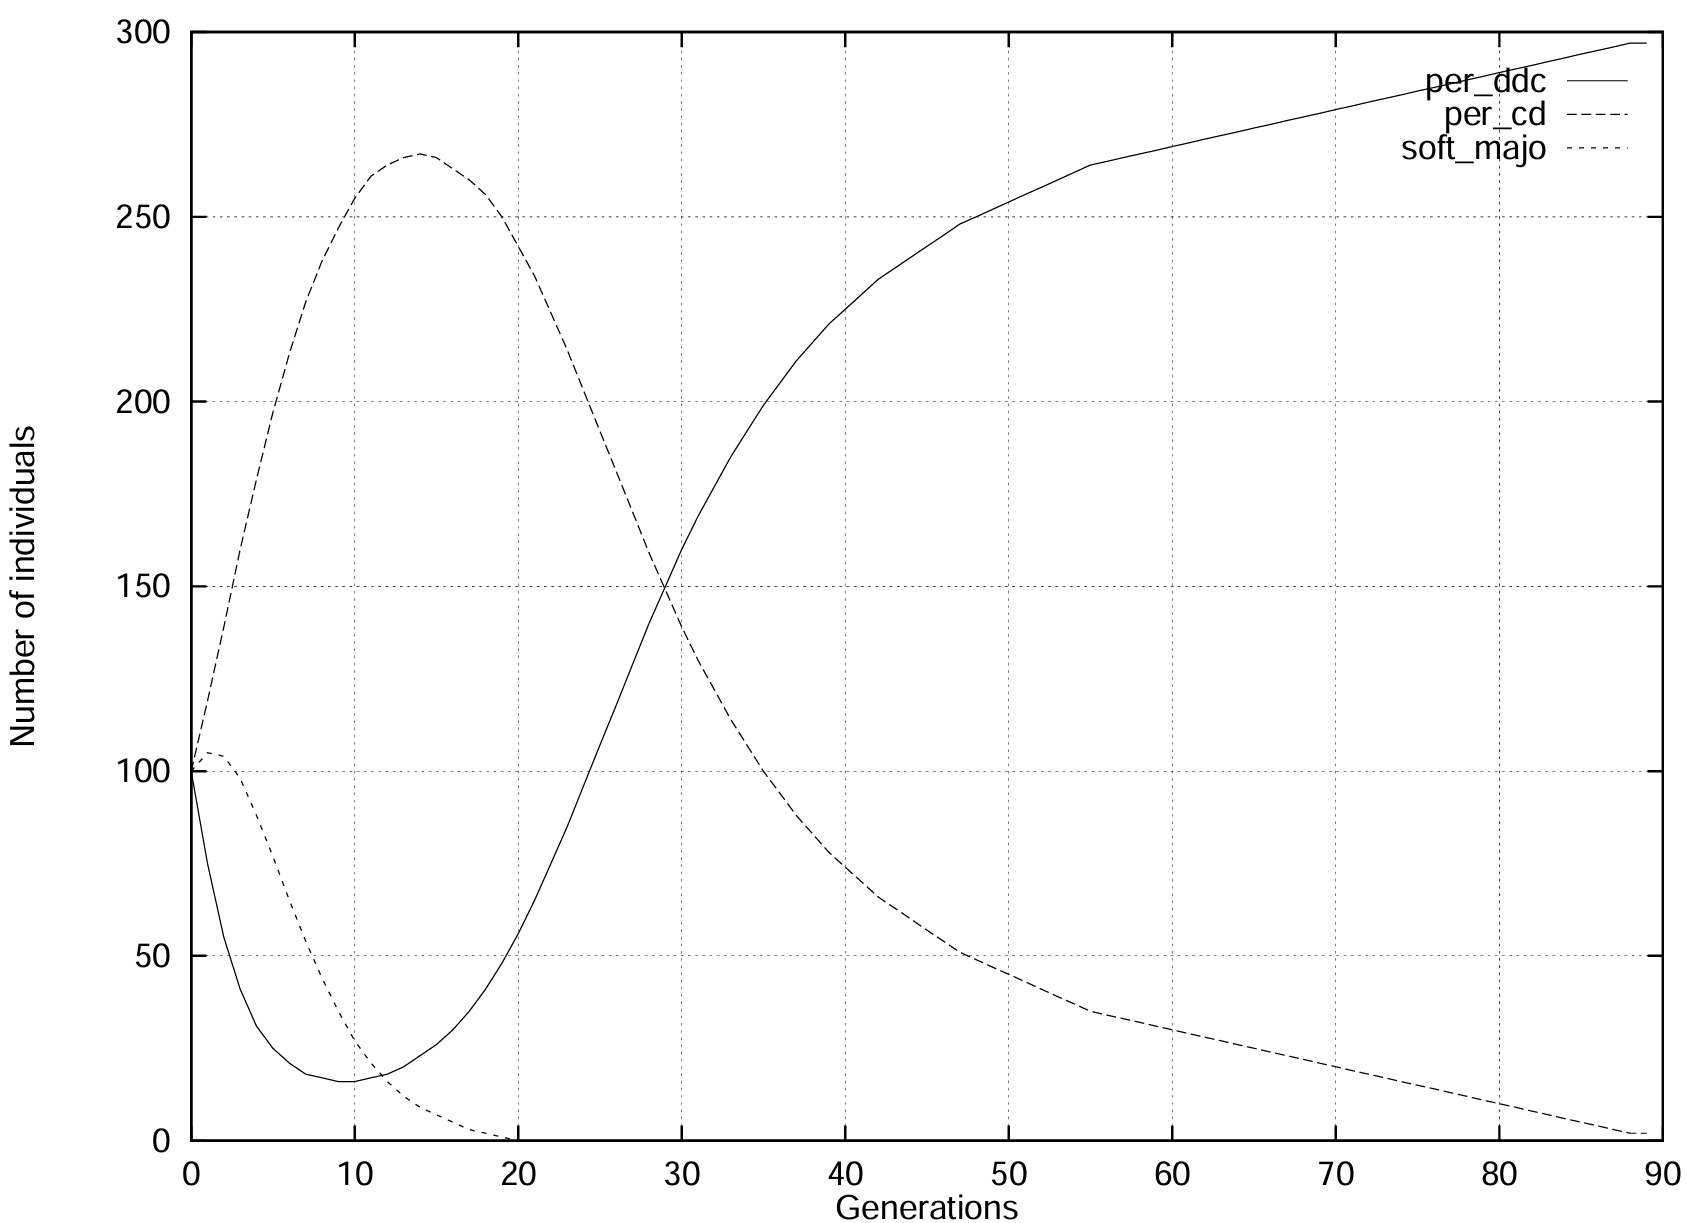
\includegraphics[width=0.7\textwidth]{RefPaperFigures/fig1.jpeg}\par\vspace{0.5em}
		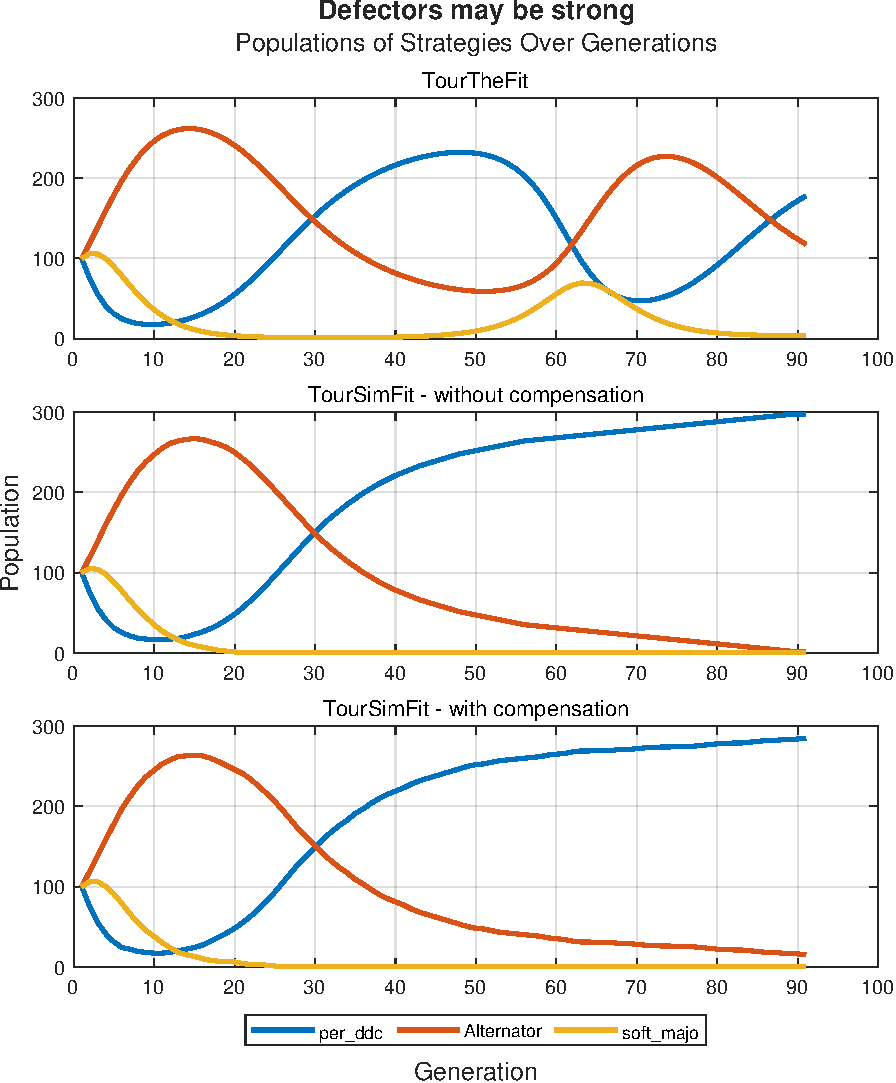
\includegraphics[width=0.7\textwidth]{Defectors may be strong.pdf}
	    \caption{1st Simulation - Defectors may be strong}
	    \label{fig:Defectors may be strong}
	\end{figure}
\subsubsection{2nd Simulation - Monotonous Convergence}
From now on, the results are presented for the simulations used by Mathieu et al. to classify the graphs into 5 categories, the first of which (Figure~\ref{fig:Monotonous Convergence}) is the monotonous convergence of populations. This is the most common form that emerges, as the oscillations presented below are quite sensitive to initial conditions. The results of both the theoretical analysis and the two simulations are identical to those of Mathieu et al., with the only difference being a slightly different final population in the case of \texttt{compensation}, which is again due to the stochastic element. However, the ranking of the strategies remains the same. Run example02 of the Examples folder (after reading Quickstart guide) to recreate the figure.

	\begin{figure}[h]
	    \centering
		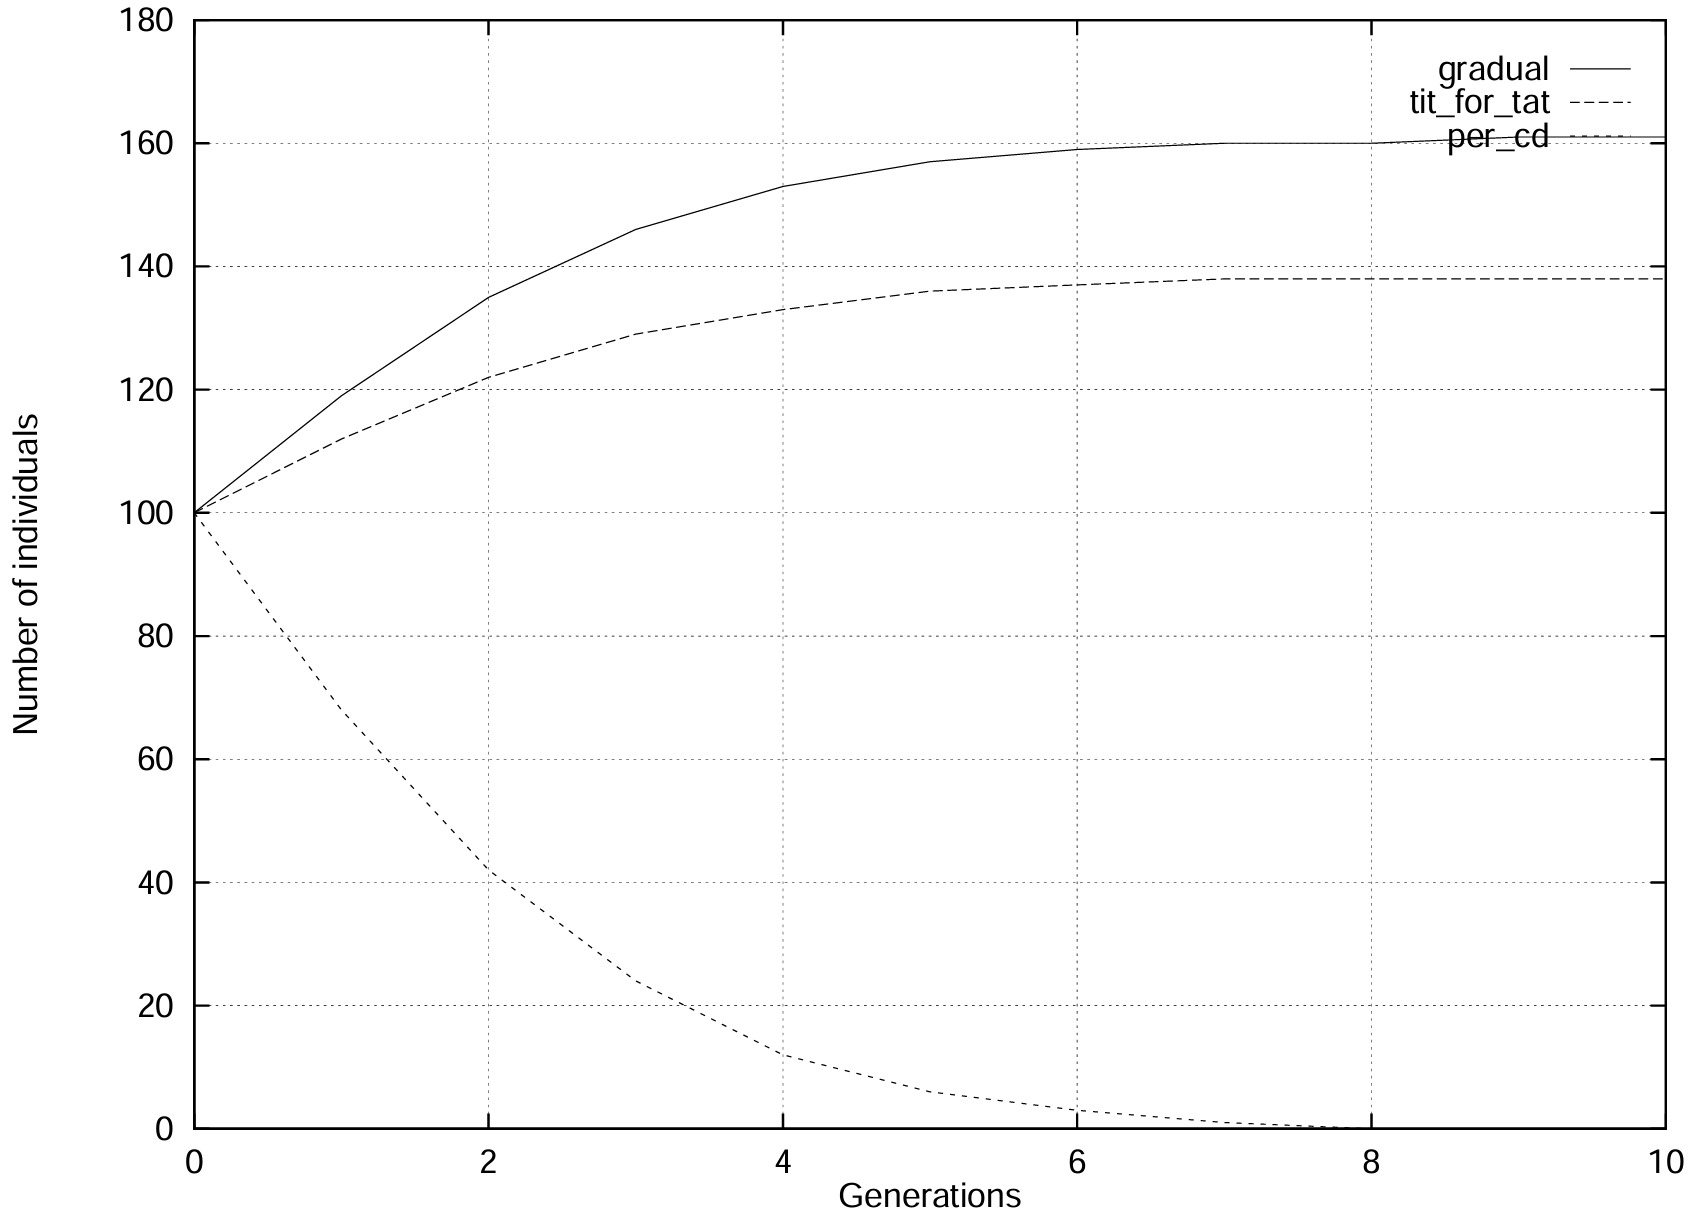
\includegraphics[width=0.7\textwidth]{RefPaperFigures/fig2.jpeg}\par\vspace{0.5em}
	    \includegraphics[width=0.7\textwidth]{Monotonous Convergence.pdf}
	    \caption{2nd Simulation - Monotonous Convergence}
	    \label{fig:Monotonous Convergence}
	\end{figure}
\subsubsection{3rd Simulation - Attenuated Oscillatory movements}
The next category of results from the paper is the diminishing oscillations of populations (Figure~\ref{fig:Attenuated oscillatory movements}). The results in this case are identical to those of Mathieu et al. for all three cases presented. The initial populations in this particular case are quite large, so the one or two players that randomly oppose in the \texttt{compensation} scenario do not significantly affect the trajectory of the function. Run example03 of the Examples folder (after reading Quickstart guide) to recreate the figure.

	\begin{figure}[h]
	    \centering
		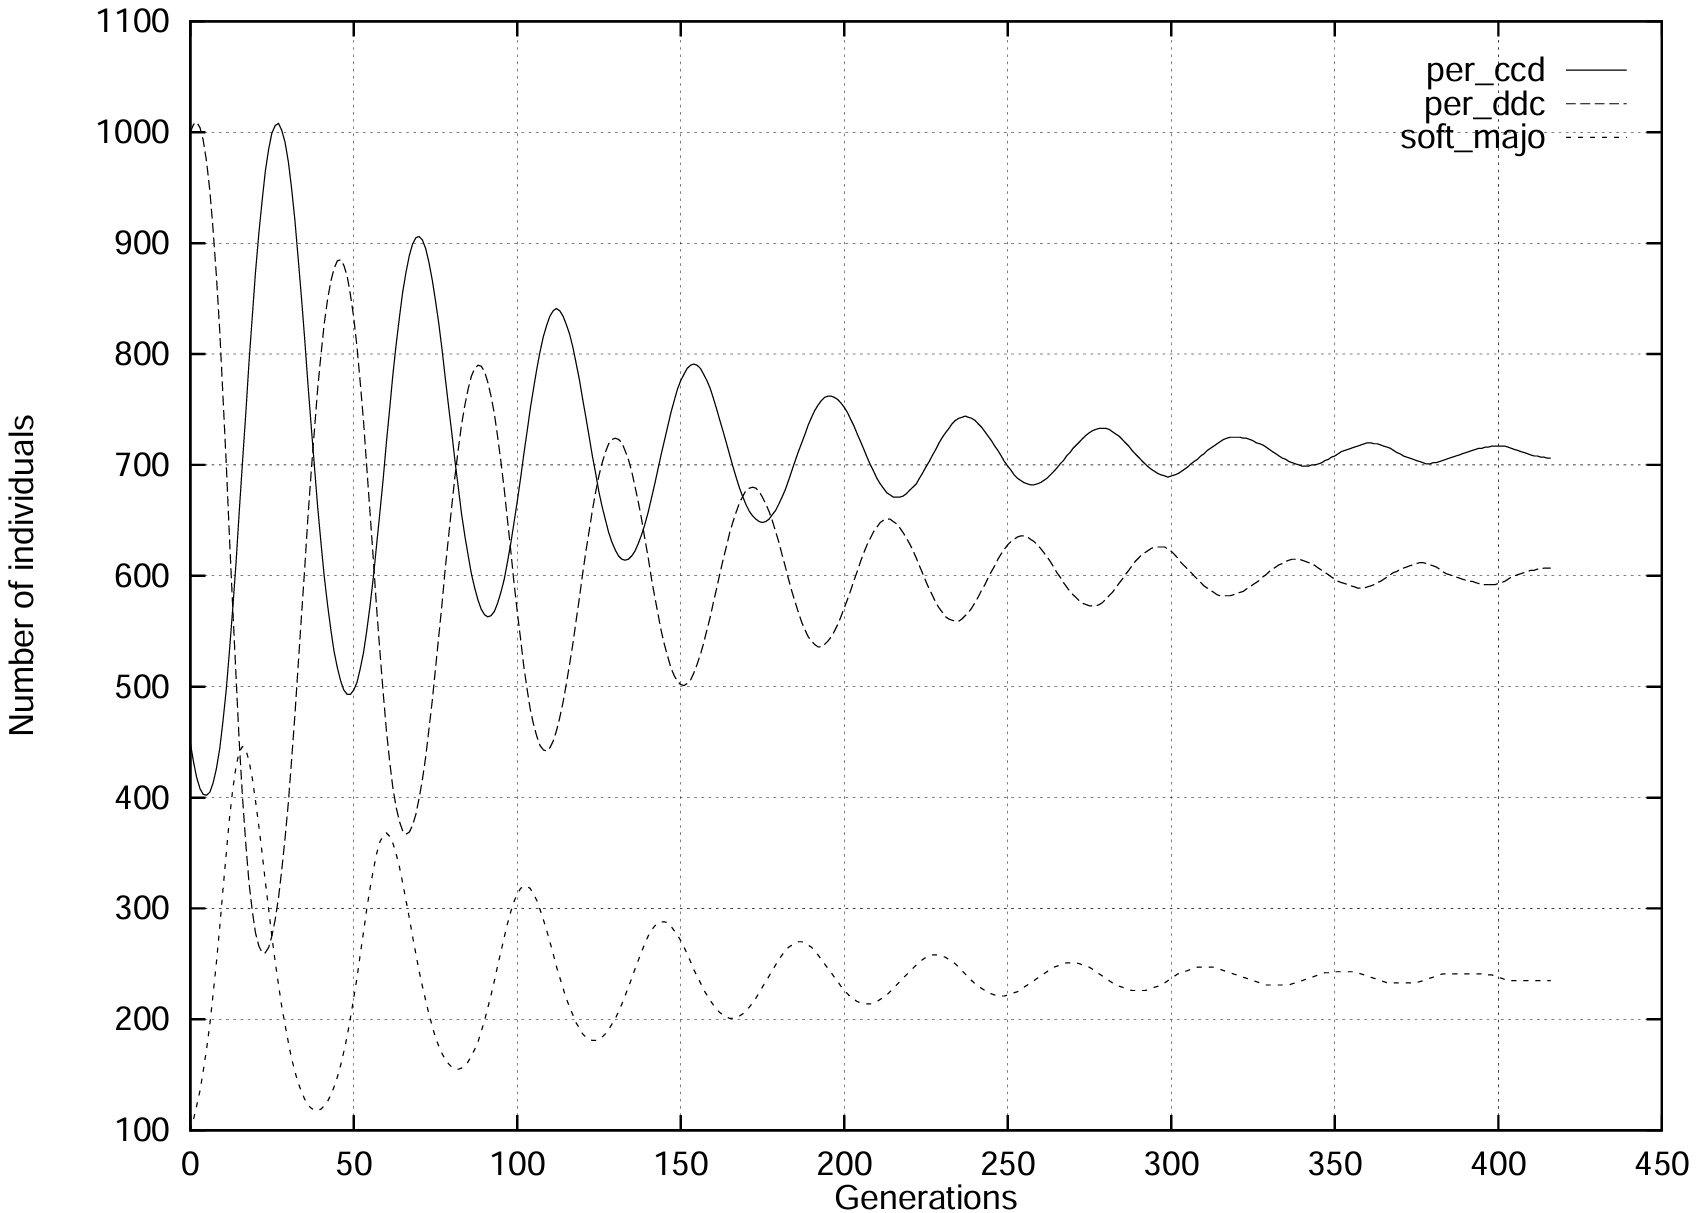
\includegraphics[width=0.7\textwidth]{RefPaperFigures/fig3.jpeg}\par\vspace{0.5em}
	    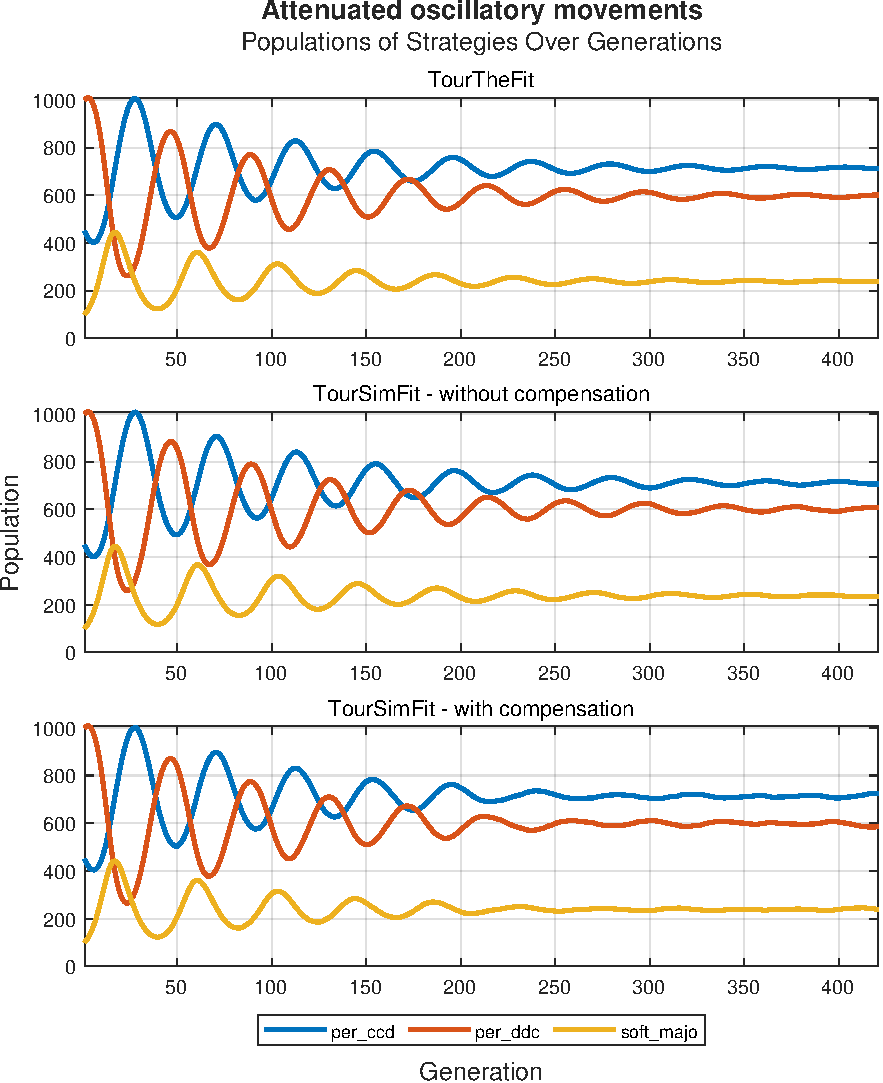
\includegraphics[width=0.7\textwidth]{Attenuated oscillatory movements.pdf}
	    \caption{3rd Simulation - Attenuated oscillatory movements}
	    \label{fig:Attenuated oscillatory movements}
	\end{figure}
\subsubsection{4th Simulation - Periodic movements}
The third case is the appearance of periodic movements/oscillations (Figure~\ref{fig:Periodic movements}), without an increase or decrease in the amplitude of the oscillations. This behavior generally appears when there are three strategies with a "rock-paper-scissors" logic: the 1st "beats" the 2nd, which "beats" the 3rd, which in turn "beats" the 1st. In this particular case, \texttt{per\_ccd} beats \texttt{soft\_majo}, which beats \texttt{per\_ddc}, which beats \texttt{per\_ccd}. With appropriate initial populations, the following results are observed. The theoretical analysis shows that the oscillation actually fades — it is a diminishing oscillation as before. This is due to the fact that in discrete cases, such as these simulations, it becomes certain through suitable choices that the system will return to a previous state, and thus repetition/oscillation will occur. However, in the theoretical analysis, this does not happen (due to the "infinity" of states because of decimal numerics), and thus the oscillation is damped. The \texttt{TourSimFit} function without \texttt{compensation} again yields results identical to those of Mathieu et al., while the case with \texttt{compensation}, although visually less appealing, also captures the oscillation, even with noticeable noise due to randomness (the amplitudes of the oscillations are small, so even the addition of one or two extra players has a noticeable effect). Run example04 of the Examples folder (after reading Quickstart guide) to recreate the figure.

	\begin{figure}[h]
	    \centering
		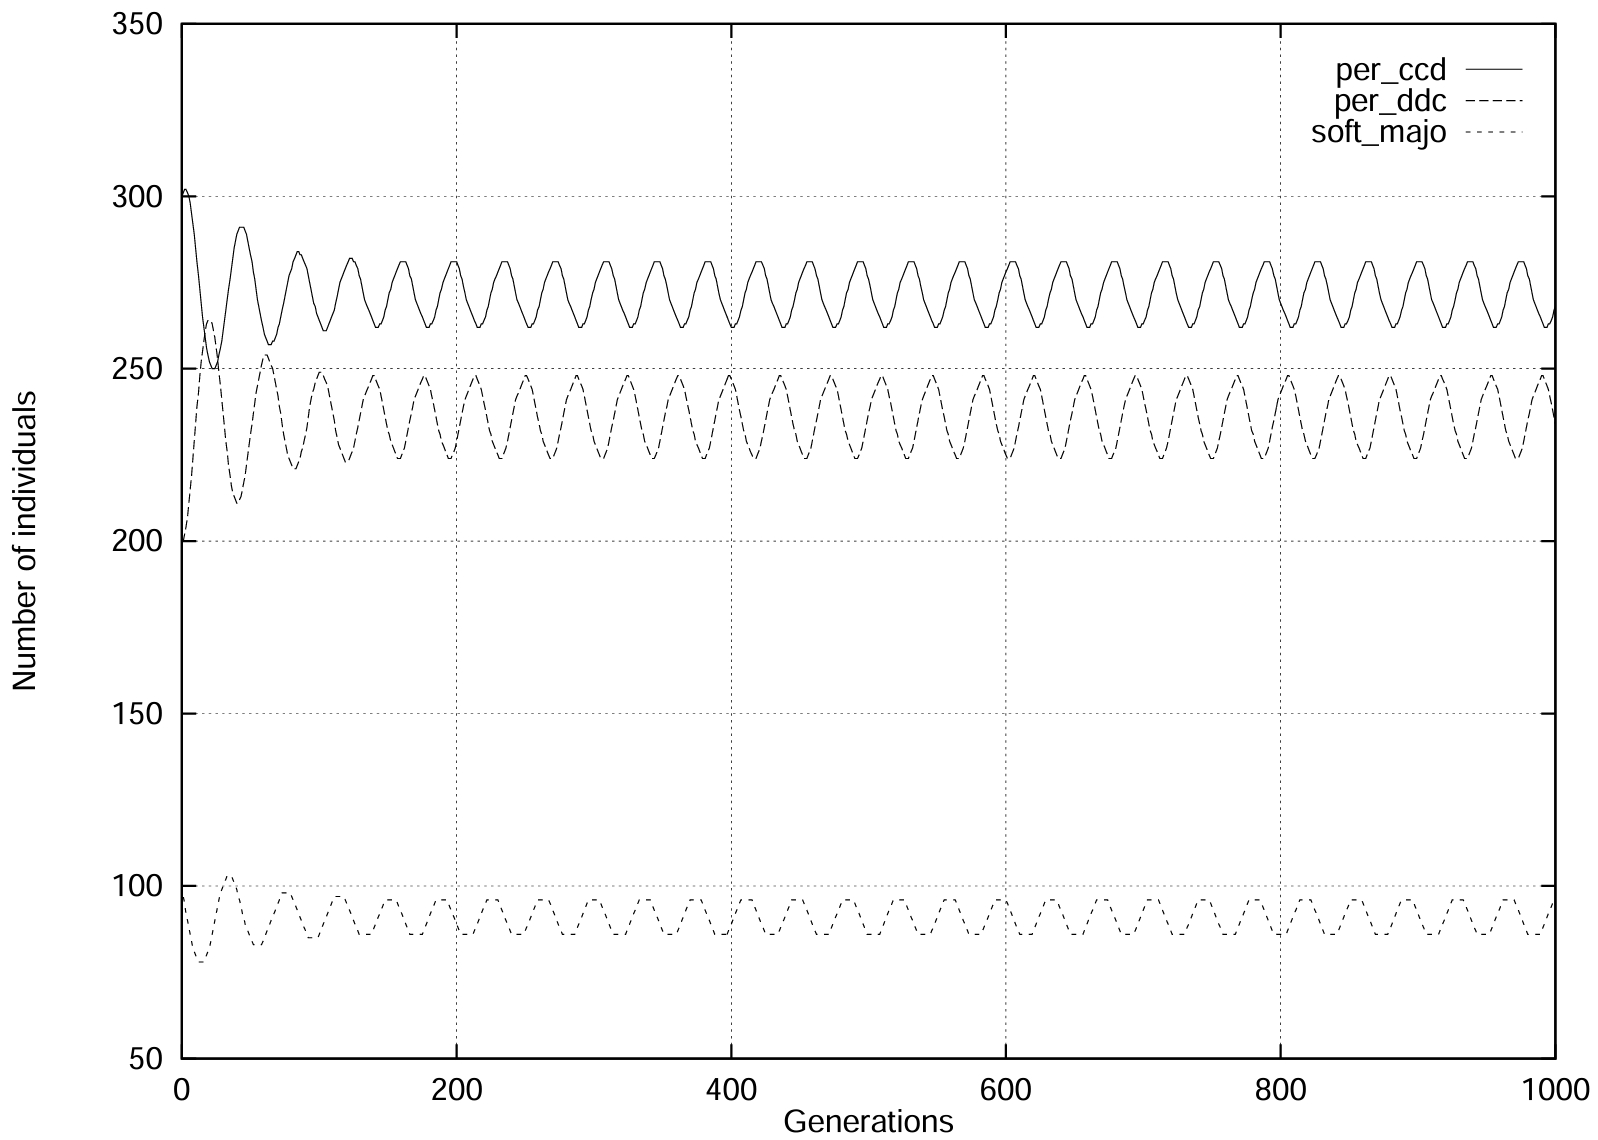
\includegraphics[width=0.7\textwidth]{RefPaperFigures/fig4.jpeg}\par\vspace{0.5em}
	    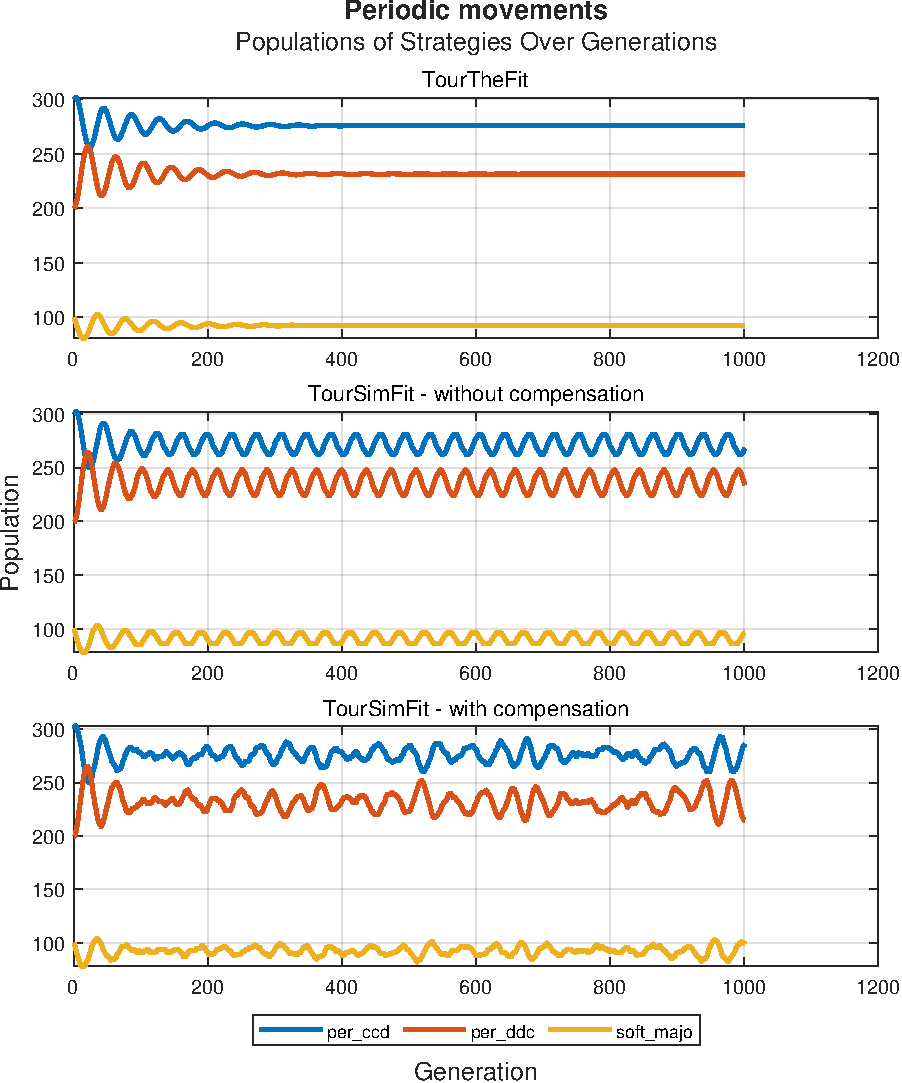
\includegraphics[width=0.7\textwidth]{Periodic movements.pdf}
	    \caption{4th Simulation - Periodic movements}
	    \label{fig:Periodic movements}
	\end{figure}
\subsubsection{5th Simulation - Increasing oscillations}
One of the most unexpected cases is that of increasing oscillations (Figure~\ref{fig:Increasing oscillations}). With an appropriate choice of the payoff matrix, strategies, and initial populations, this phenomenon can be observed.

 A result very similar to that of the paper was observed in the case of \texttt{TourSimFit} without \texttt{compensation}. However, for the cases of \texttt{TourTheFit} and \texttt{TourSimFit} with \texttt{compensation}, diminishing oscillations are observed, revealing two truths about the cases of increasing oscillations. First, they arise from populations capable of exhibiting normal oscillations, with a suitable modification of the payoff matrix. Second, they are particularly sensitive cases that collapse back into normal or diminishing oscillations with even a slight modification of the dynamics (such as the logic of \texttt{compensation}). It is quite possible that for an appropriate choice of \( B \), the cases of \texttt{TourTheFit} and \texttt{TourSimFit} with \texttt{compensation} could also transform into increasing oscillations, but it was considered more important for this work to present this divergence in the results. Run example05 of the Examples folder (after reading Quickstart guide) to recreate the figure.

	\begin{figure}[h]
	    \centering
		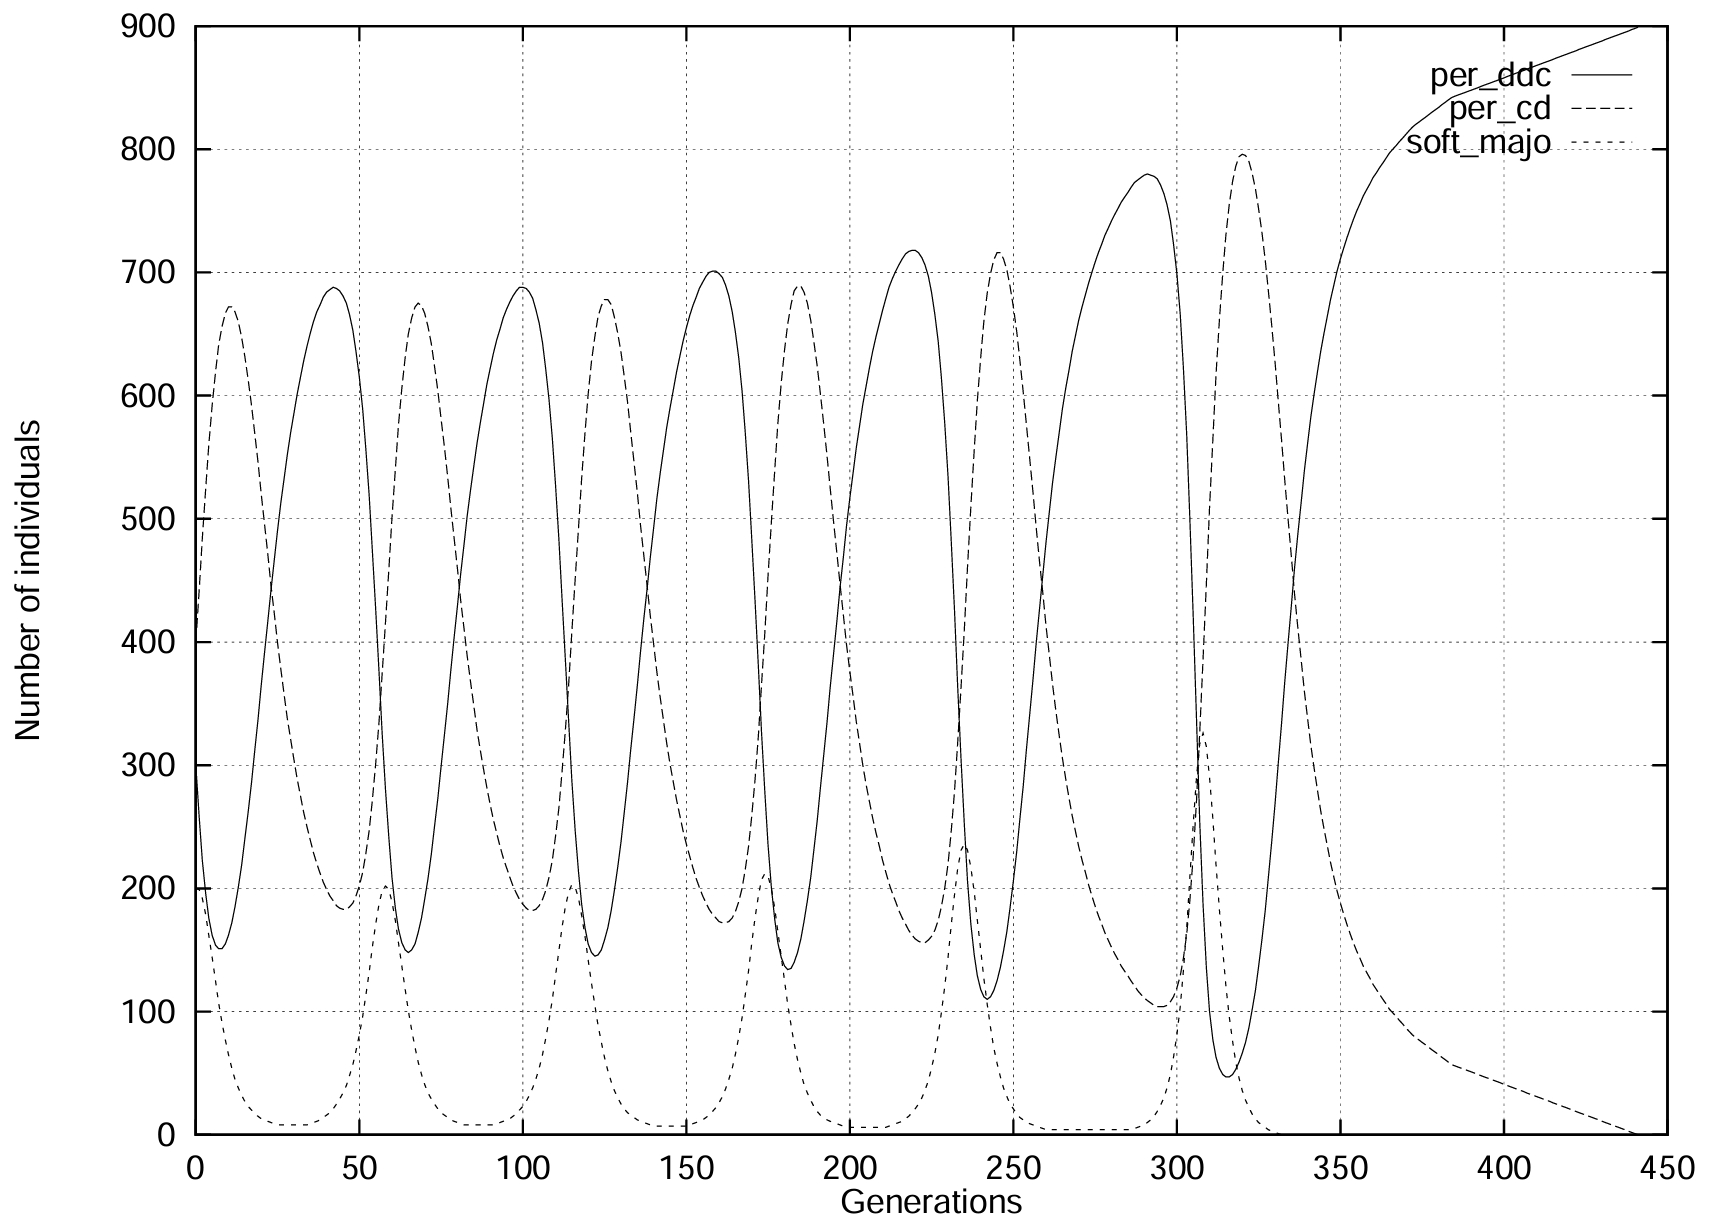
\includegraphics[width=0.7\textwidth]{RefPaperFigures/fig5.jpeg}\par\vspace{0.5em}
	    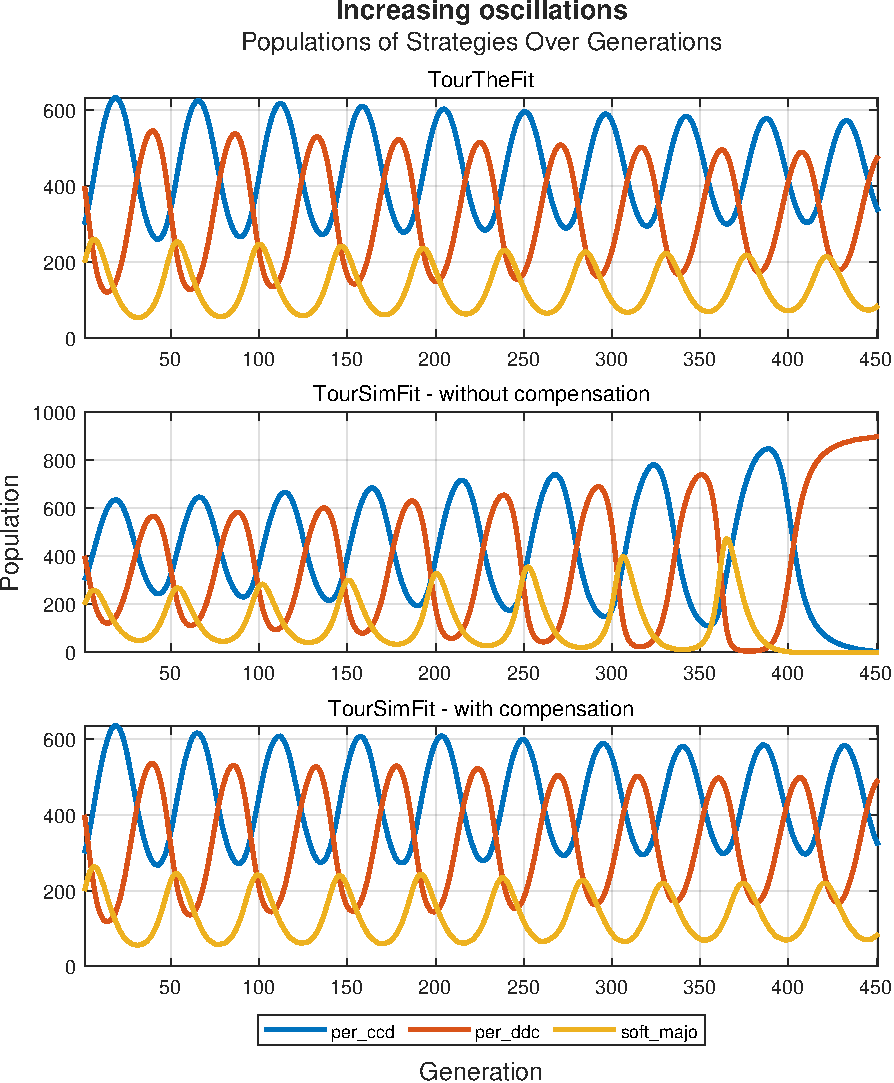
\includegraphics[width=0.7\textwidth]{Increasing oscillations.pdf}
	    \caption{5th Simulation - Increasing oscillations}
	    \label{fig:Increasing oscillations}
	\end{figure}
\subsubsection{6th Simulation - Chaos/Disordered oscillations}
The last case presented in the paper is that of disordered oscillations (Figure~\ref{fig:Disordered oscillations}). The authors of the paper rightly hesitate to characterize it as a truly chaotic case because, due to the discrete nature of the simulation, any such behavior after a sufficient number of generations either reaches equilibrium or simply repeats. However, the results of this particular simulation appear quite chaotic. Again, the case of \texttt{TourSimFit} without \texttt{compensation} fully matches the results of the paper. In contrast, due to the sensitivity of the phenomenon, the cases of the theoretical analysis and the actual simulation with \texttt{compensation} differ significantly, as they do not exhibit the chaotic behavior around generation 140 as in the case of the paper. Nevertheless, they predict the survival of the \texttt{per\_ccccd} and \texttt{Prober} strategies, as well as the values toward which the populations in the \texttt{TourSimFit} case without simulation seem to tend. Run example06 of the Examples folder (after reading Quickstart guide) to recreate the figure.

	\begin{figure}[h]
	    \centering
		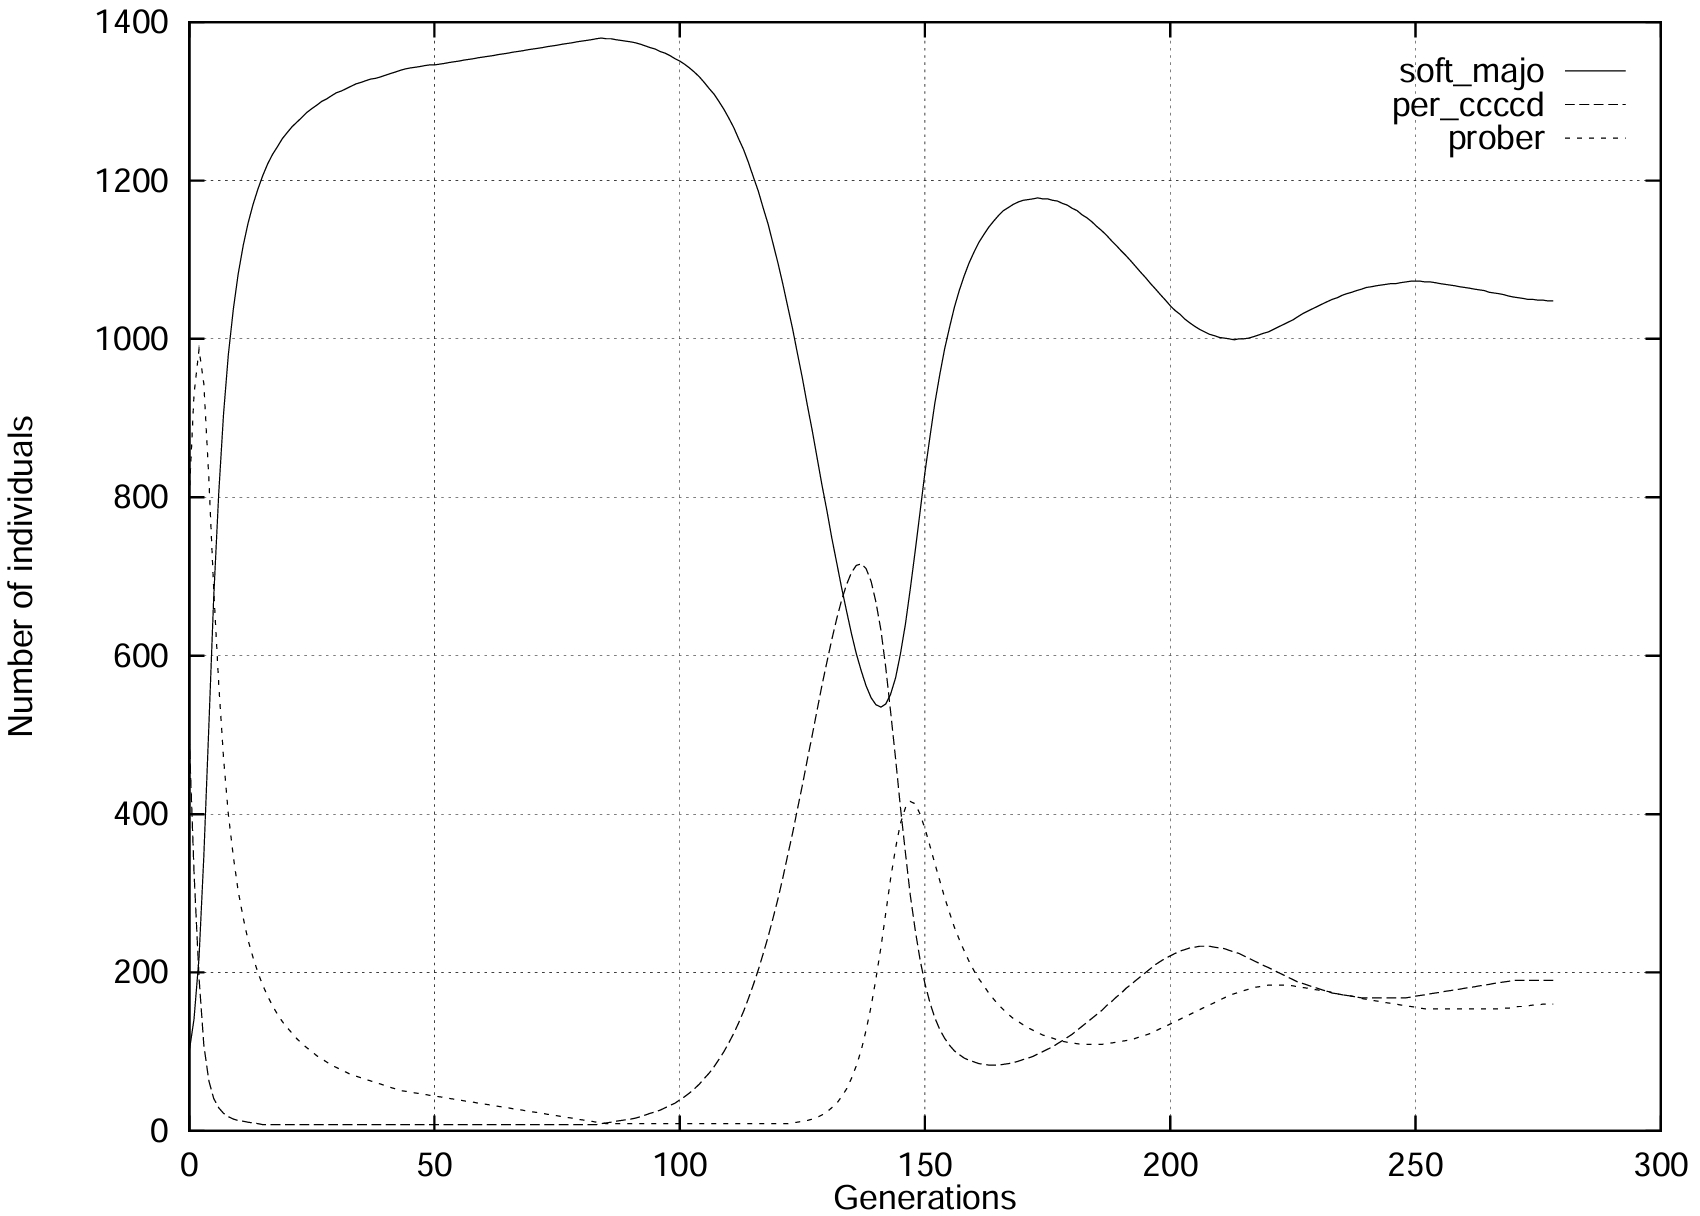
\includegraphics[width=0.7\textwidth]{RefPaperFigures/fig6.jpeg}\par\vspace{0.5em}
	    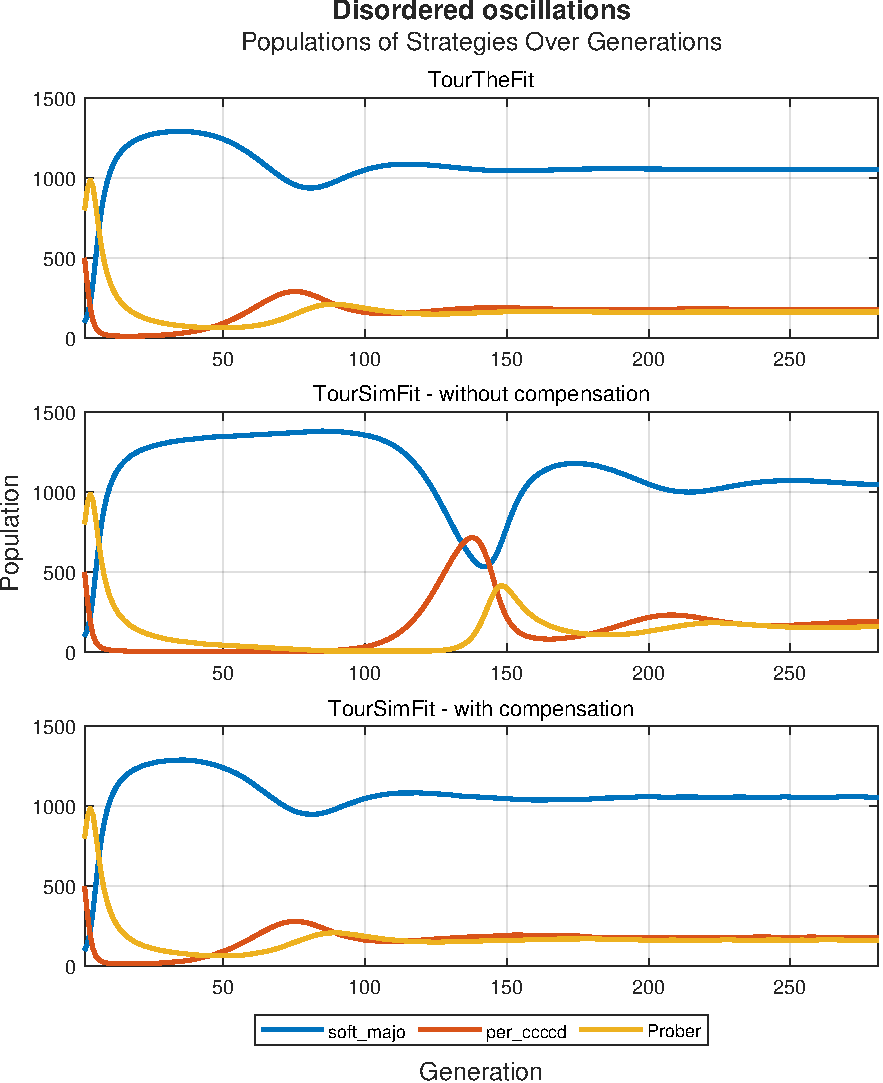
\includegraphics[width=0.7\textwidth]{Disordered oscillations.pdf}
	    \caption{6th Simulation - Disordered oscillations}
	    \label{fig:Disordered oscillations}
	\end{figure}

\subsubsection{7th Simulation - Sensitivity of dynamics to population's size - First Simulation}
From now on, the simulations showcase the sensitivity of the results to the initial conditions of the examples. Again, the results presented are compared to the results of Mathieu et al and any differences are discussed. The first simulation aims to present the sensitivity of the dynamics to the initial population's size for each strategy. More specifically, the same set of strategies can lead to many different forms of dynamics occuring, depending on the population of each of the strategy. This should not come as a surprise, as even in the previous examples the strategies used were often the same, with the differences in dynamics being caused by different initial populations. In this first example (Figure~\ref{fig:Sensitivity of dynamics to population's size - First Simulation}), the result is a periodic movement, which is also recreated in the TourSimFit without compensation, as well as (mostly) in the TourSimFit with compensation. However, the theoretical result of TourTheFit is an attenuated oscillation, as in the case of the Figure~\ref{fig:Periodic movements}, for the same reasons as before. Run example07 of the Examples folder (after reading Quickstart guide) to recreate the figure.

	\begin{figure}[h]
	    \centering
		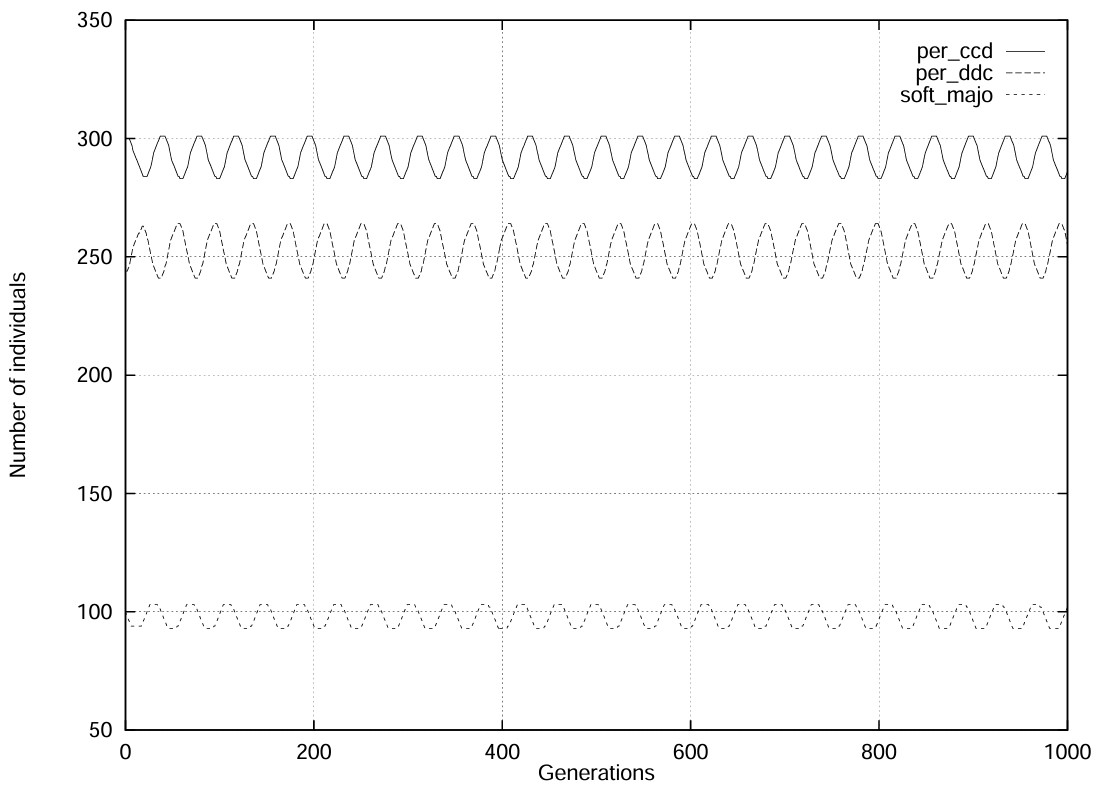
\includegraphics[width=0.7\textwidth]{RefPaperFigures/fig7a.jpeg}\par\vspace{0.5em}
	    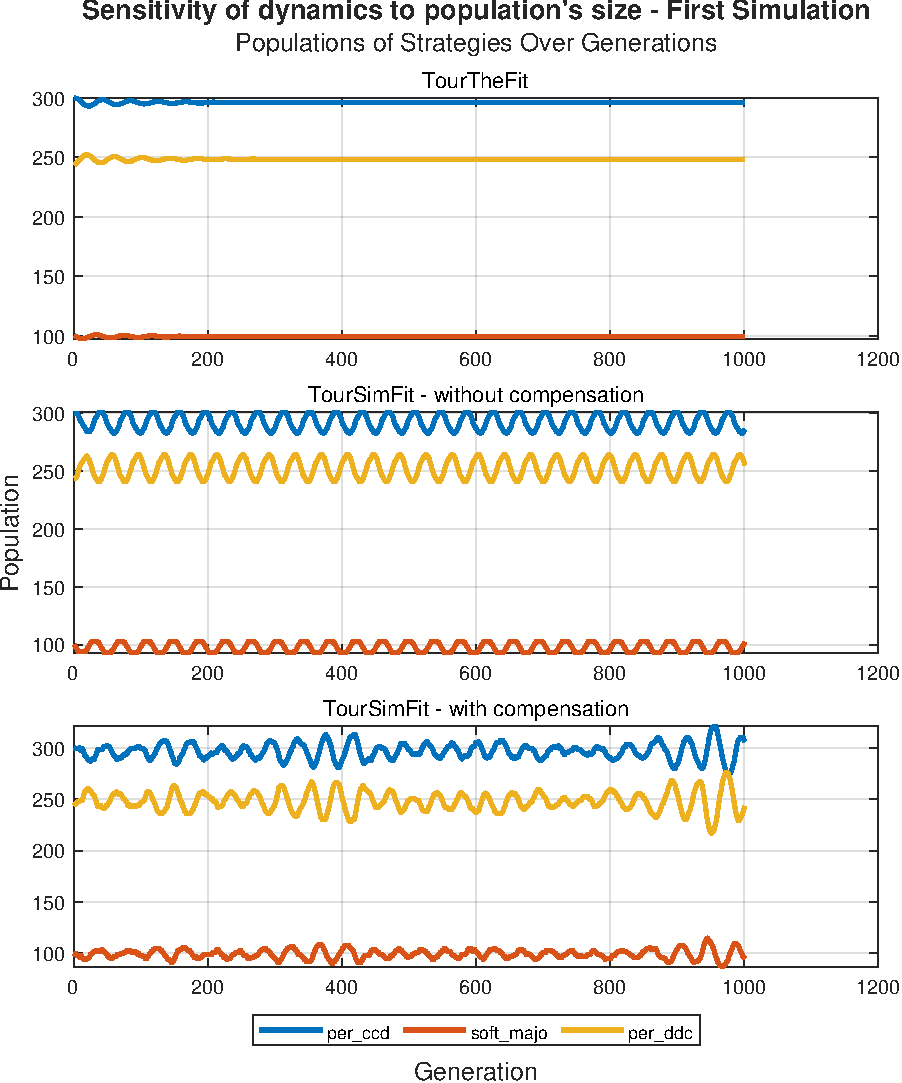
\includegraphics[width=0.7\textwidth]{Sensitivity of dynamics to population's size - First Simulation.pdf}
	    \caption{7th Simulation - Sensitivity of dynamics to population's size - First Simulation}
	    \label{fig:Sensitivity of dynamics to population's size - First Simulation}
	\end{figure}
\subsubsection{8th Simulation - Sensitivity of dynamics to population's size - Second Simulation}
The second example of the showcase of the sensitivity of the dynamics to the population's size shows a monotonous convergence that is caused by a slight differentiation in the initial population vector of the previous simulation. The only difference between this simulation and the previous one is one extra \texttt{per\_ddc} added, which ends up being enough to change the resulting dynamics completely. This is recreated (Figure~\ref{fig:Sensitivity of dynamics to population's size - Second Simulation}) in the case of TourSimFit without compensation. However, in the cases of TourTheFit there appears to still be a slight attenuated oscillation, meaning the convergence is not monotonous, and in the case of the TourSimFit with compensation the result is still a periodic movement, obviously caused by the random element of this method. Thus, we observe a large sensitivity of the dynamics to the repartition method of the population, which is also discussed in a later example. Run example08 of the Examples folder (after reading Quickstart guide) to recreate the figure.

	\begin{figure}[h]
	    \centering
		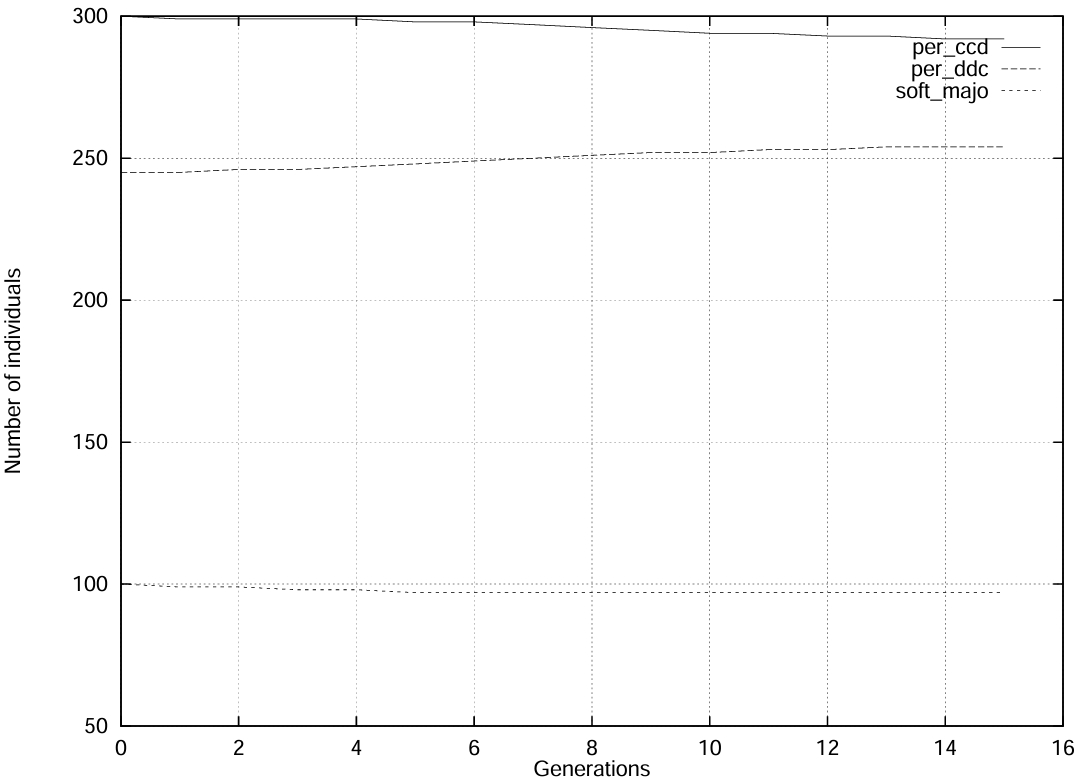
\includegraphics[width=0.7\textwidth]{RefPaperFigures/fig7b.jpeg}\par\vspace{0.5em}
	    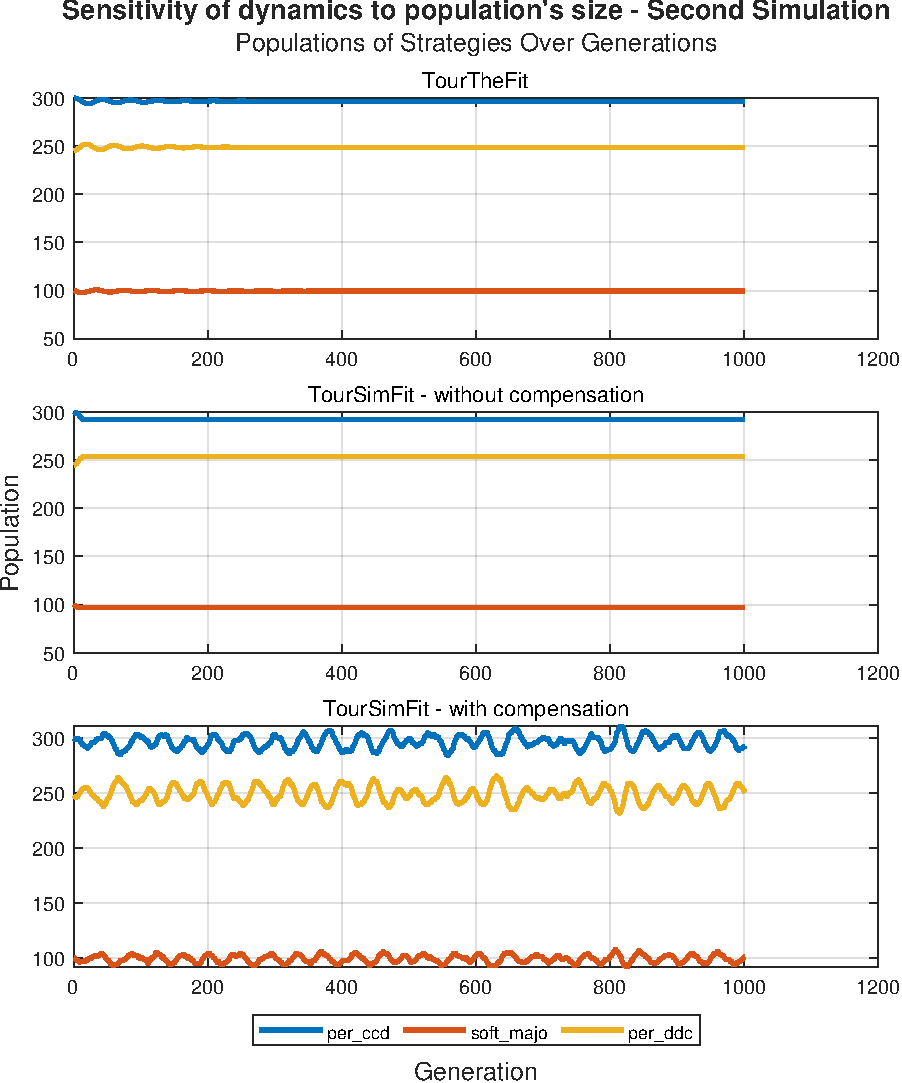
\includegraphics[width=0.7\textwidth]{Sensitivity of dynamics to population's size - Second Simulation.pdf}
	    \caption{8th Simulation - Sensitivity of dynamics to population's size - Second Simulation}
	    \label{fig:Sensitivity of dynamics to population's size - Second Simulation}
	\end{figure}
\subsubsection{9th Simulation - Sensitivity of winner to population's size - First Simulation}
The second case presented is the sensitivity of the winner to the population's size, with winner being the strategy that ends up having the most members of the population at the end of the simulation. This may not be obvious at first; we have seen a lot of cases where the change in dynamics is clearly visible but the ensuing winner still remains the same in most cases. The first example (Figure~\ref{fig:Sensitivity of winner to population's size - First Simulation}) shows an initial population that ultimately announces \texttt{per\_ddc} as the winning strategy; the winner is recreated by each of our own methods, however the dynamics in the case of TourTheFit are visibly different, due to the population of \texttt{soft\_majo} never actually dying out and thus making the \texttt{Alternator} strategy more viable (as we covered, \texttt{Alternator} is the perfect counter to \texttt{soft\_majo}). Run example09 of the Examples folder (after reading Quickstart guide) to recreate the figure.
	\begin{figure}[h]
	    \centering
		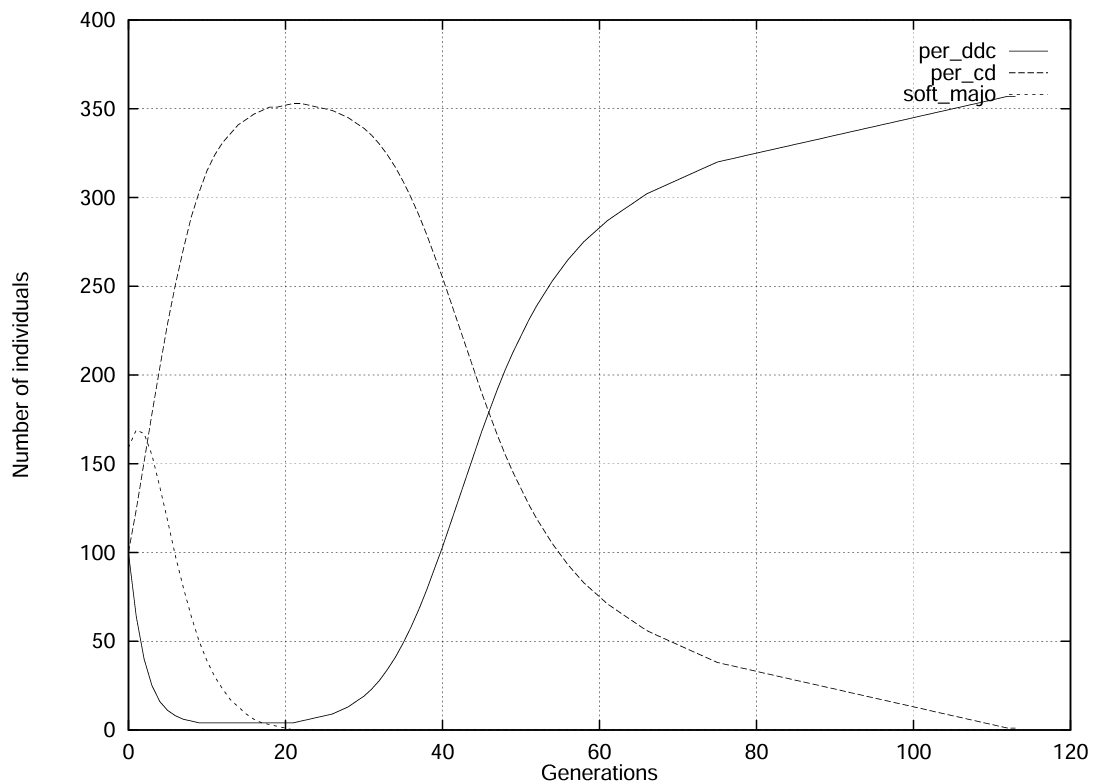
\includegraphics[width=0.7\textwidth]{RefPaperFigures/fig8a.jpeg}\par\vspace{0.5em}
	    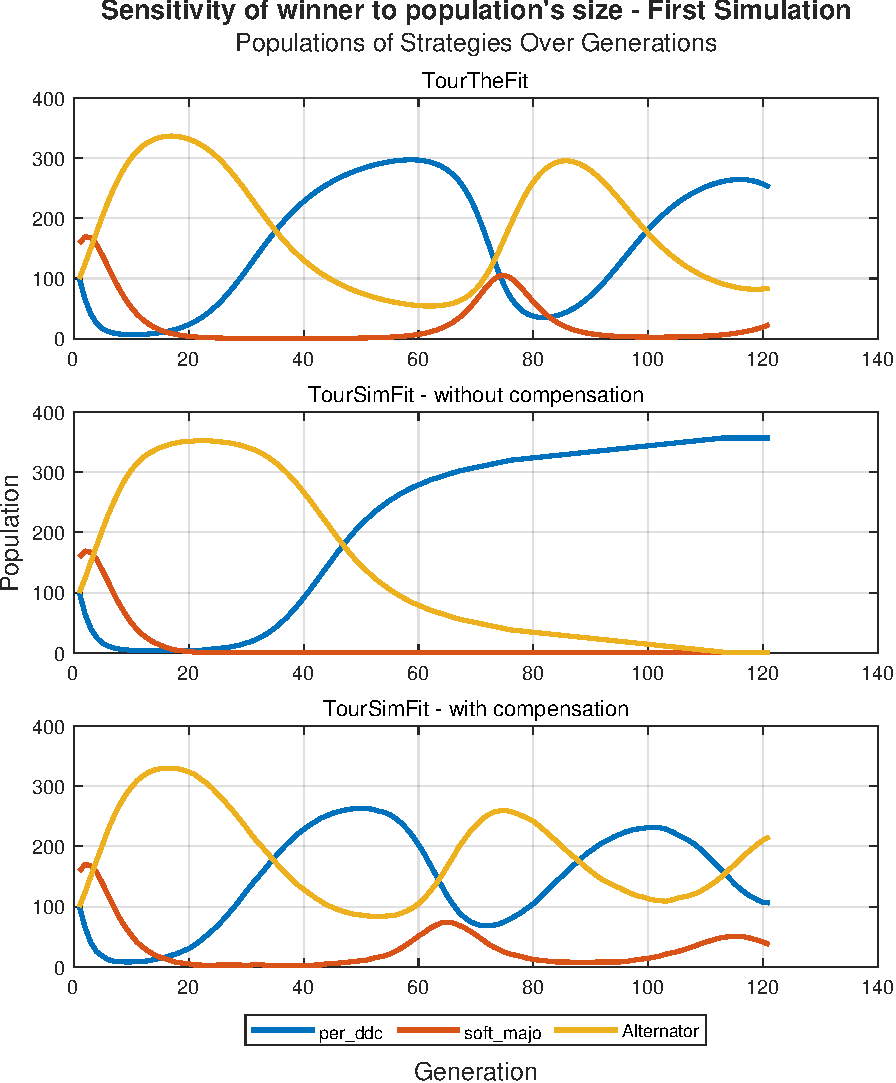
\includegraphics[width=0.7\textwidth]{Sensitivity of winner to population's size - First Simulation.pdf}
	    \caption{9th Simulation - Sensitivity of winner to population's size - First Simulation}
	    \label{fig:Sensitivity of winner to population's size - First Simulation}
	\end{figure}
\subsubsection{10th Simulation - Sensitivity of winner to population's size - Second Simulation}
The second part of the sensitivity of winner to population's size showcase adds one \texttt{soft\_majo} participant to the initial population, making \texttt{Alternator} the winner. The results (Figure~\ref{fig:Sensitivity of winner to population's size - Second Simulation}) are recreated in the case of TourSimFit without compensation. However, in the cases of TourTheFit and TourSimFit with compensation, \texttt{Alternator} does not seem to be the decisive winner of the simulation, since at the end of the simulation there is still a rising population of \texttt{per\_ddc}, strategy which does better versus \texttt{Alternator}, meaning that the eventual winner would be \texttt{per\_ddc}. This in turn is caused by the fact that the population of \texttt{per\_ddc} is not eliminated in these two cases, thus making a comeback possible. Note that, as Mathieu et al suggest, the modified strategy never wins (unless if it was already the winner). Run example10 of the Examples folder (after reading Quickstart guide) to recreate the figure.
	\begin{figure}[h]
	    \centering
		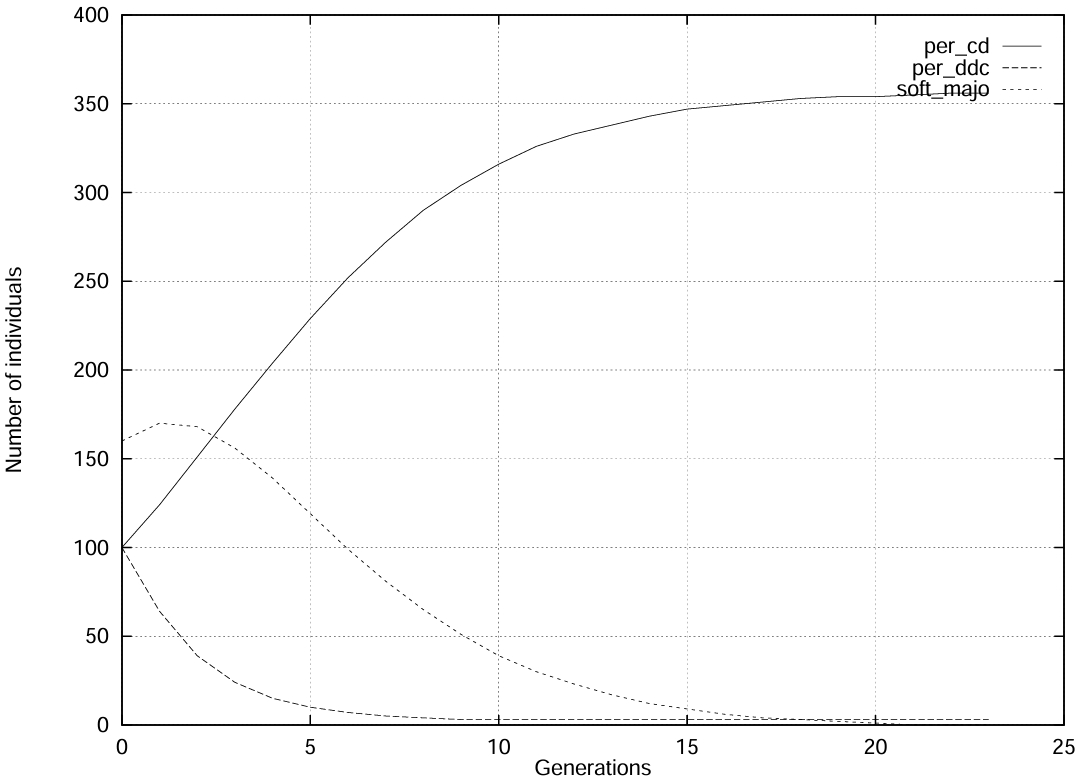
\includegraphics[width=0.7\textwidth]{RefPaperFigures/fig8b.jpeg}\par\vspace{0.5em}
	    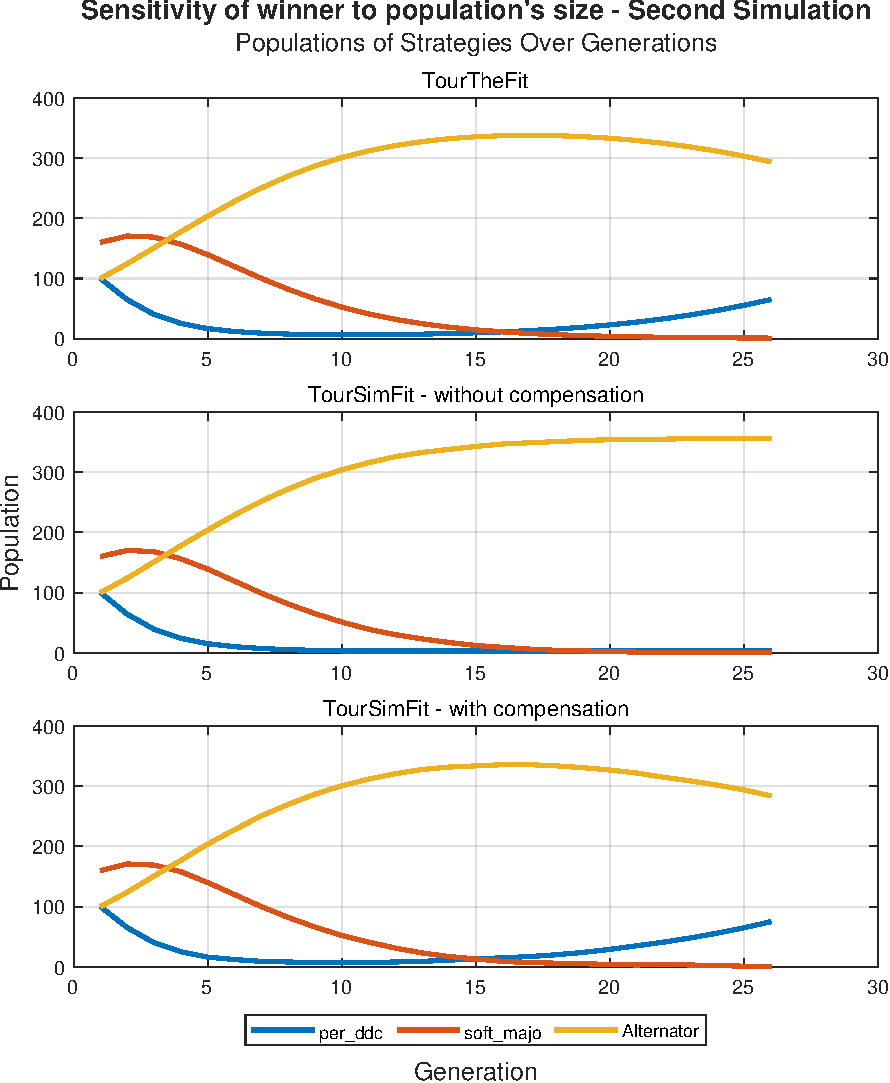
\includegraphics[width=0.7\textwidth]{Sensitivity of winner to population's size - Second Simulation.pdf}
	    \caption{10th Simulation - Sensitivity of winner to population's size - Second Simulation}
	    \label{fig:Sensitivity of winner to population's size - Second Simulation}
	\end{figure}
\subsubsection{11th Simulation - Sensitivity to game length - First Simulation}
The next aspect of initial conditions studied is the game length, meaning the number of rounds each match between two players lasts. As it turns out, periodic strategies like most studied in this project are sensitive to the game length, because of the varying ``winner'' of each match based on the amount of rounds played. In the first part, each match lasts 7 rounds and the result is a periodic movement. This is also recreated (Figure~\ref{fig:Sensitivity to game length - First Simulation}) in the case of TourSimFit without compensation, but it again becomes an attenuated oscillatory movement for the cases of TourTheFit and TourSimFit with compensation, for the same reasons as discussed multiple times (a true periodic movement without making rounding errors in some generations is very sensitive). Run example11 of the Examples folder (after reading Quickstart guide) to recreate the figure.
	\begin{figure}[h]
	    \centering
		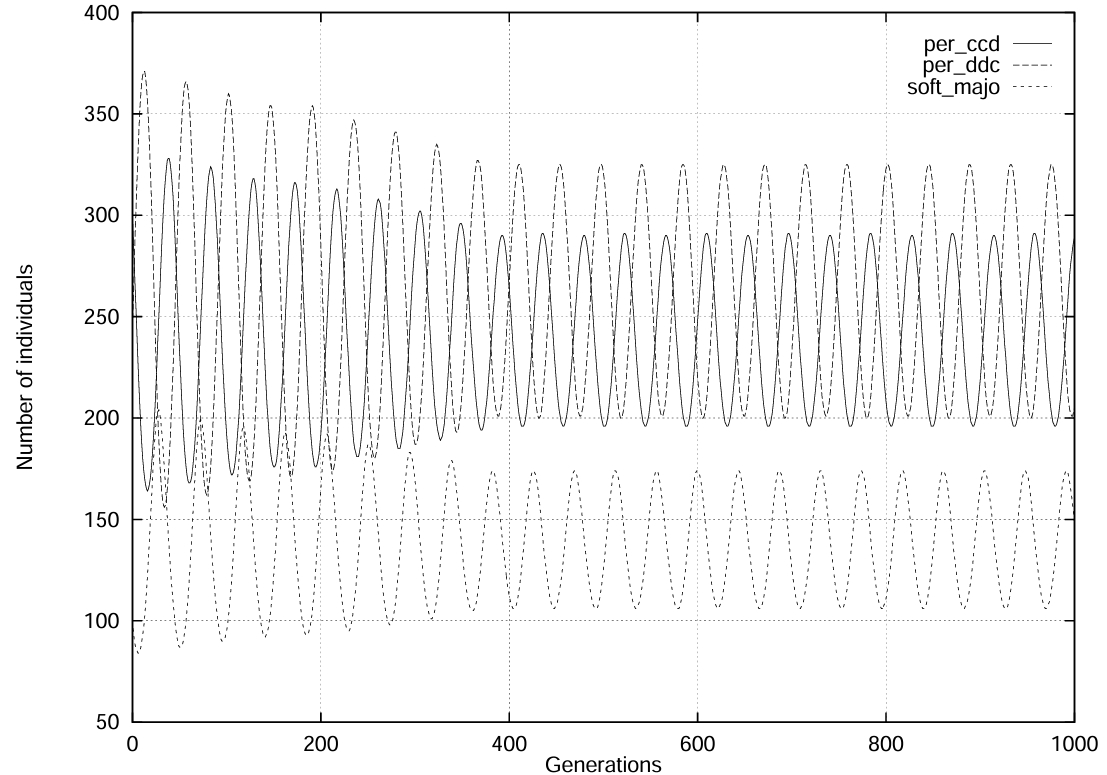
\includegraphics[width=0.7\textwidth]{RefPaperFigures/fig9a.jpeg}\par\vspace{0.5em}
	    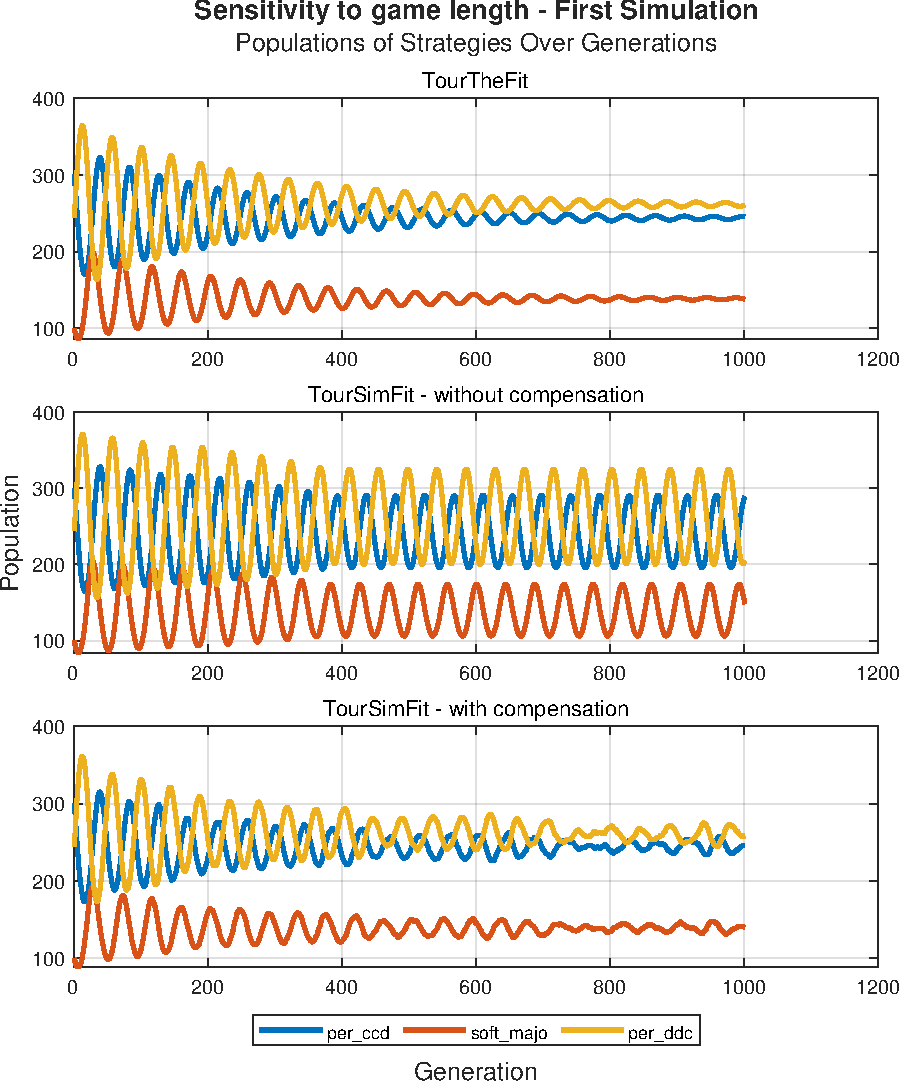
\includegraphics[width=0.7\textwidth]{Sensitivity to game length - First Simulation.pdf}
	    \caption{11th Simulation - Sensitivity to game length - First Simulation}
	    \label{fig:Sensitivity to game length - First Simulation}
	\end{figure}
\subsubsection{12th Simulation - Sensitivity to game length - Second Simulation}
The second simulation of this part changes only the number of rounds played each match to 6. This results in an attenuated oscillatory movement, which is recreated (Figure~\ref{fig:Sensitivity to game length - Second Simulation}) by every function of our own. Thus, it is shown that the dynamics, as well as the eventual winner (since a periodic movement like the one showcased in the previous example has no official winner) are sensitive to the game length, especially when periodic strategies are used. This happens because, for example, in a 6 round game \texttt{per\_ccd} does not lose as hard to \texttt{per\_ddc} as in the case of a 7 round game (it suffers one less ``effective'' defection, meaning an opponent defection met with cooperation). These slight modifications to the score of each match change the fitness score of each strategy enough to create visible changes to the outcome. Run example12 of the Examples folder (after reading Quickstart guide) to recreate the figure.
	\begin{figure}[h]
	    \centering
		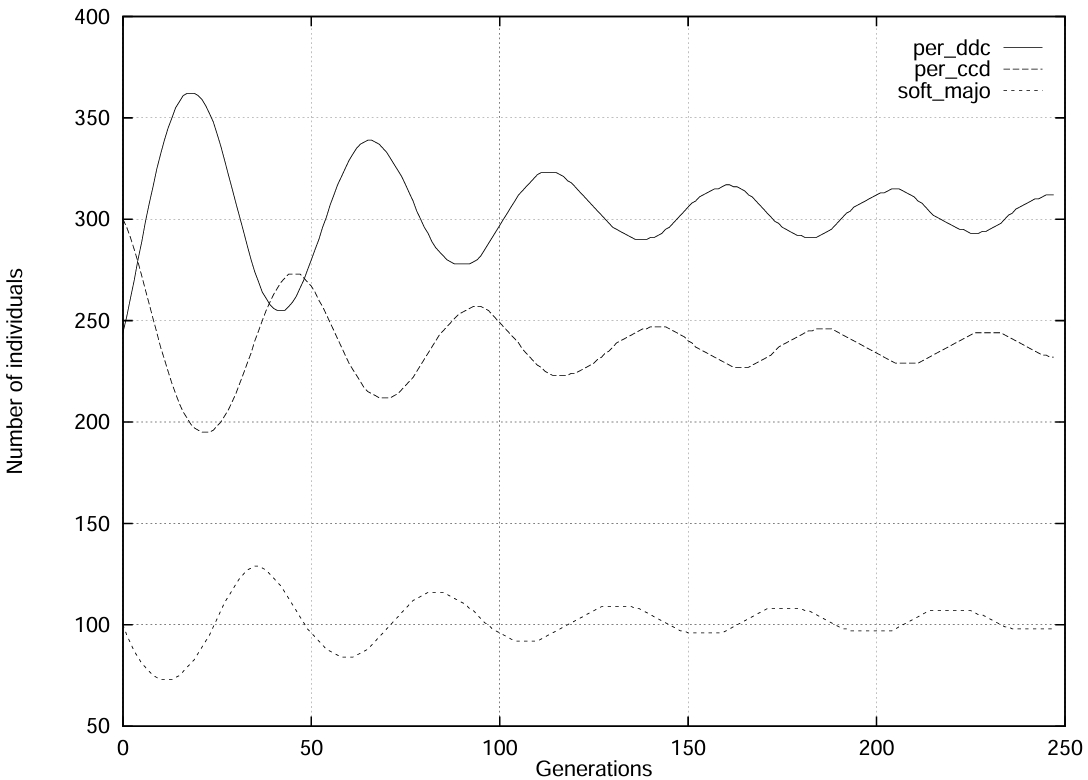
\includegraphics[width=0.7\textwidth]{RefPaperFigures/fig9b.jpeg}\par\vspace{0.5em}
	    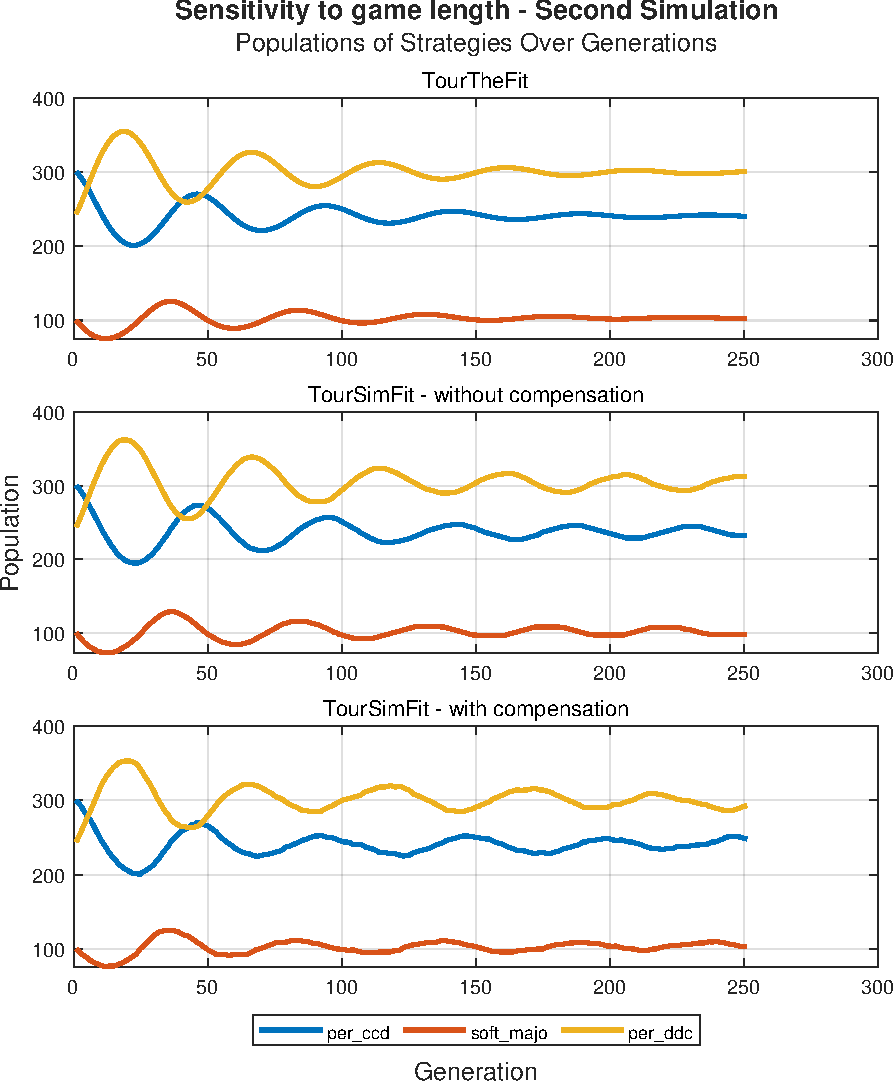
\includegraphics[width=0.7\textwidth]{Sensitivity to game length - Second Simulation.pdf}
	    \caption{12th Simulation - Sensitivity to game length - Second Simulation}
	    \label{fig:Sensitivity to game length - Second Simulation}
	\end{figure}
\subsubsection{13th Simulation - Sensitivity to CIPD payoff - First Simulation}
One other initial condition of the simulation that affects the results greatly is the CIPD payoff, meaning the payoff matrix $B$. This should not come as a surprise; the fitness of each strategy is calculated based on the scores of each match, which in turn is calculated by the payoff matrix. We have also seen in a previous example (Figure~\ref{fig:Increasing oscillations}) how even a slight change to a single element of the payoff matrix can lead to different ensuing dynamics. In the first simulation, the payoff matrix 
\[
B = \begin{bmatrix} 3 & 0 \\ 4.6 & 1 \end{bmatrix}
\] 
is chosen, resulting in increasing oscillations. This is recreated (Figure~\ref{fig:Sensitivity to CIPD payoff - First Simulation}) by all three of the functions, with a slight difference in the cases of TourTheFit and TourSimFit with compensation being that the oscillation ends quicker, as all the members of the population end up using the \texttt{per\_ccd} strategy. Run example13 of the Examples folder (after reading Quickstart guide) to recreate the figure.
	\begin{figure}[h]
	    \centering
		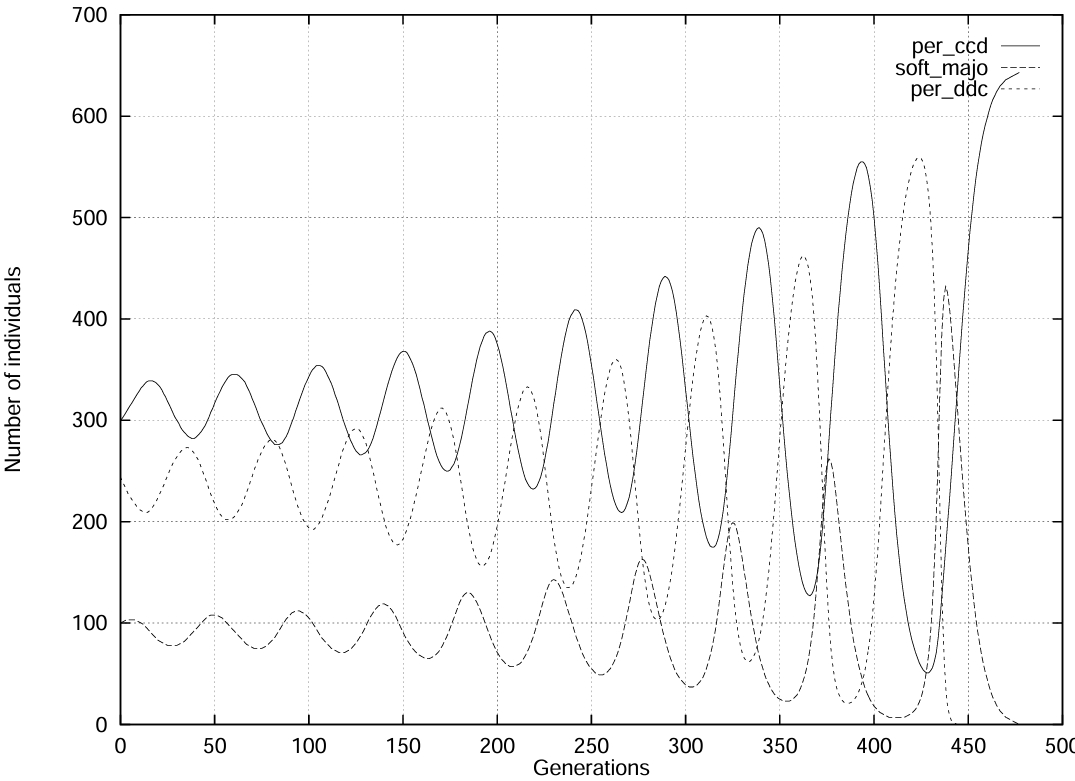
\includegraphics[width=0.7\textwidth]{RefPaperFigures/fig10a.jpeg}\par\vspace{0.5em}
	    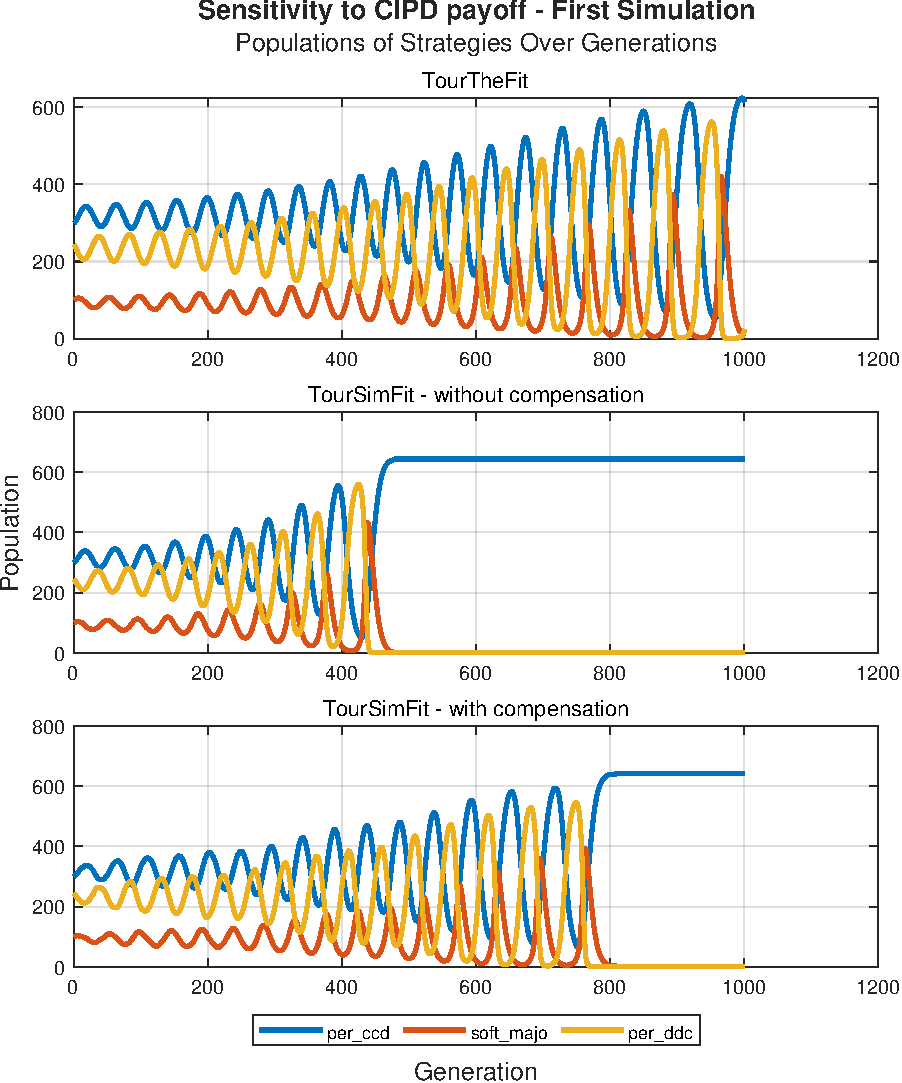
\includegraphics[width=0.7\textwidth]{Sensitivity to CIPD payoff - First Simulation.pdf}
	    \caption{13th Simulation - Sensitivity to CIPD payoff - First Simulation}
	    \label{fig:Sensitivity to CIPD payoff - First Simulation}
	\end{figure}
\subsubsection{14th Simulation - Sensitivity to CIPD payoff - Second Simulation}
In the second part of the comparison the payoff matrix is changed slightly to
\[
B = \begin{bmatrix} 3 & 0 \\ 4.7 & 1 \end{bmatrix}
\] 
resulting in periodic movements. This behavior is also presented by all functions (Figure~\ref{fig:Sensitivity to CIPD payoff - Second Simulation}), thus showing that the payoff matrix is capable of changing the resulting dynamics even with a minor adjustment. Run example14 of the Examples folder (after reading Quickstart guide) to recreate the figure.
	\begin{figure}[h]
	    \centering
		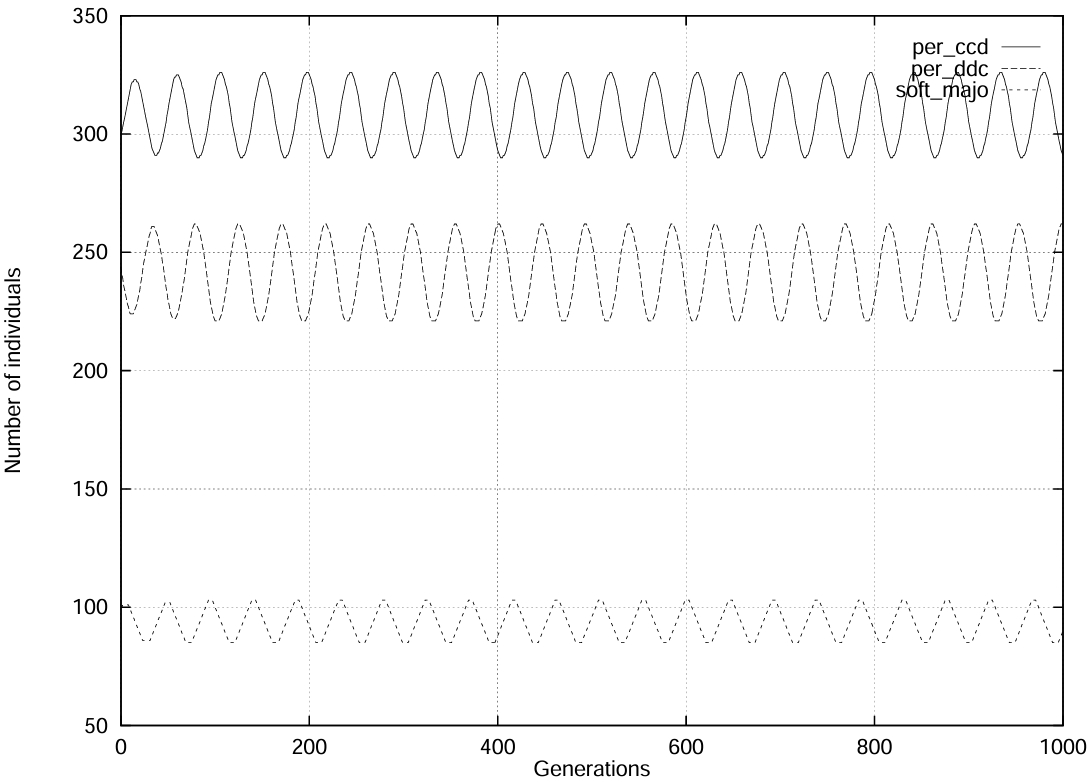
\includegraphics[width=0.7\textwidth]{RefPaperFigures/fig10b.jpeg}\par\vspace{0.5em}
	    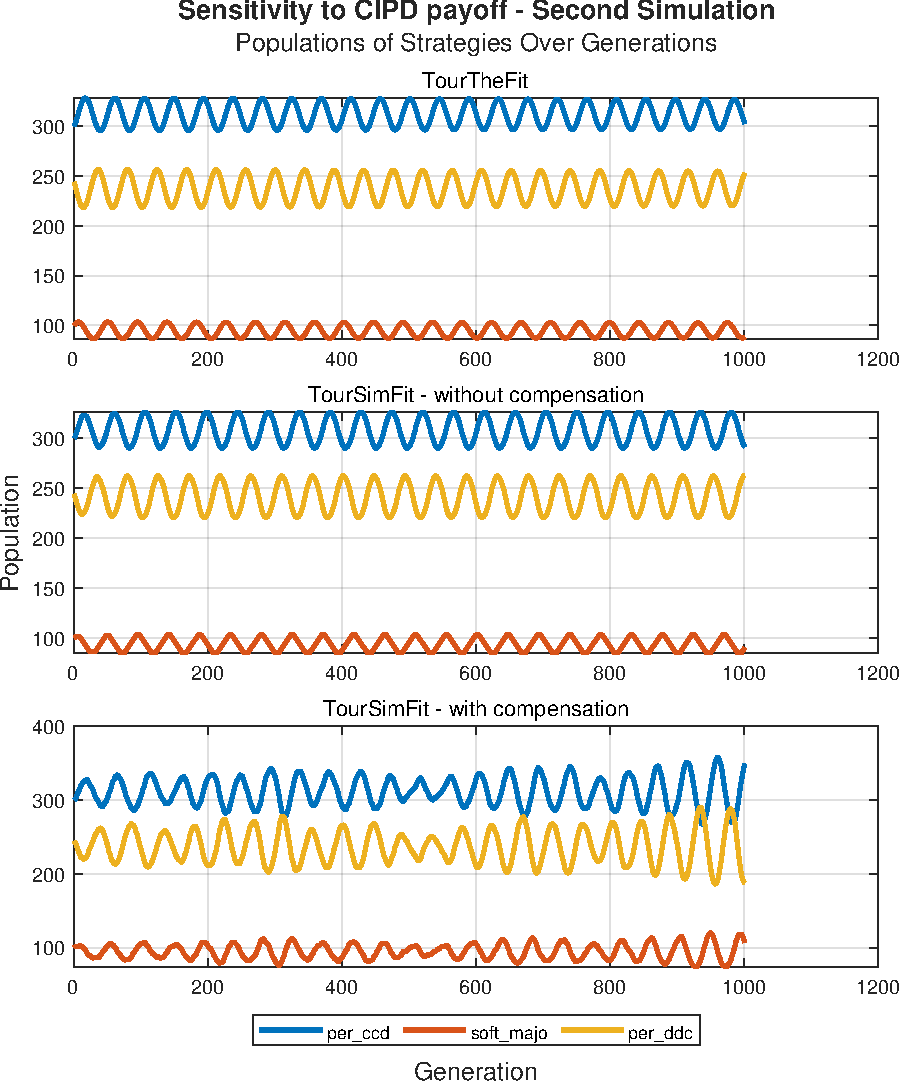
\includegraphics[width=0.7\textwidth]{Sensitivity to CIPD payoff - Second Simulation.pdf}
	    \caption{14th Simulation - Sensitivity to CIPD payoff - Second Simulation}
	    \label{fig:Sensitivity to CIPD payoff - Second Simulation}
	\end{figure}
\subsubsection{15th Simulation - Sensitivity to repartition computation method - First Simulation}
The last aspect of the simulation that is capable of producing vastly different results if altered is the repartition computation method of the simulation, meaning the way the population of the next generation is calculated. This should already be clear, since the functions of the project already have showcased different results in multiple simulations. To start, Mathieu et al calculate the population of the next generation both by rounding to the lower integer and by keeping the float number calculated (thus creating the TourTheFit function). The results are presented in Figure~\ref{fig:Sensitivity to repartition computation method - First Simulation}; the results of the plots by Mathieu et al match the results of TourSimFit with compensation and TourTheFit accordingly. Note that TourSimFit with compensation creates a similar periodic movement to the case without compensation. Also note that both plots presented by Mathieu et al are given in the same figure this time. This happens because the difference being showcased is essentially the difference between TourTheFit and TourSimFit, which we present neatly with our Figure. Run example15 of the Examples folder (after reading Quickstart guide) to recreate the figure.
	\begin{figure}[h]
	    \centering
		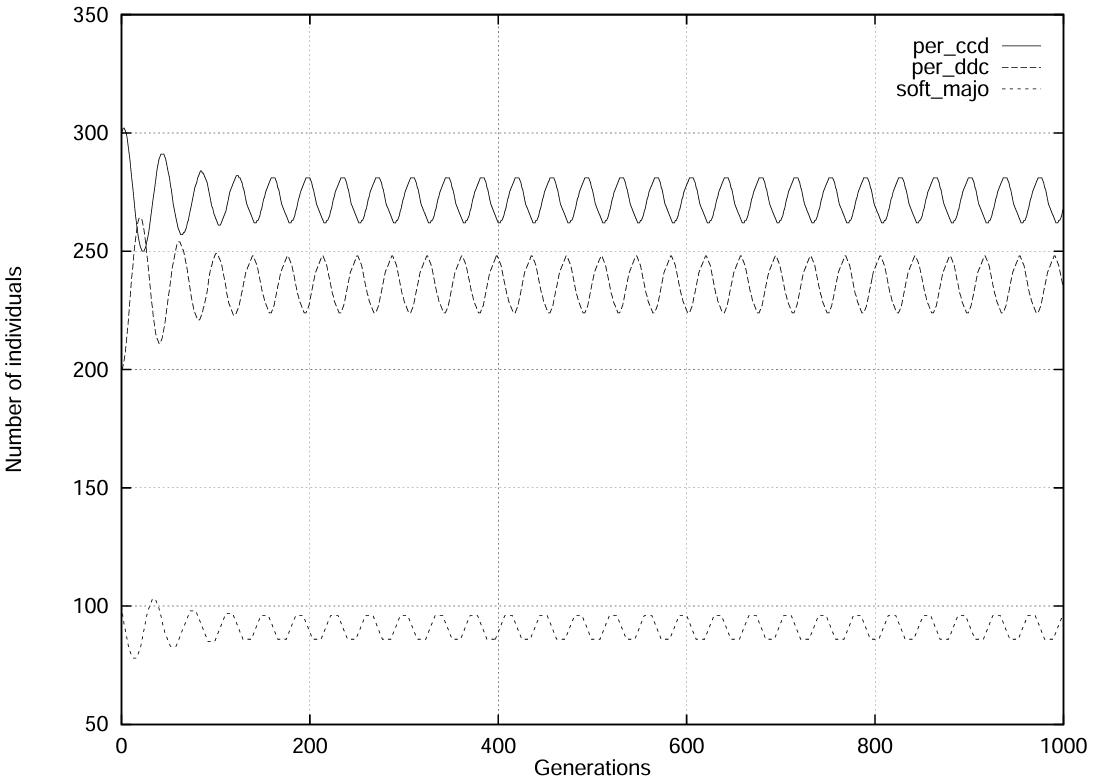
\includegraphics[width=0.49\textwidth]{RefPaperFigures/fig11a.jpeg}
		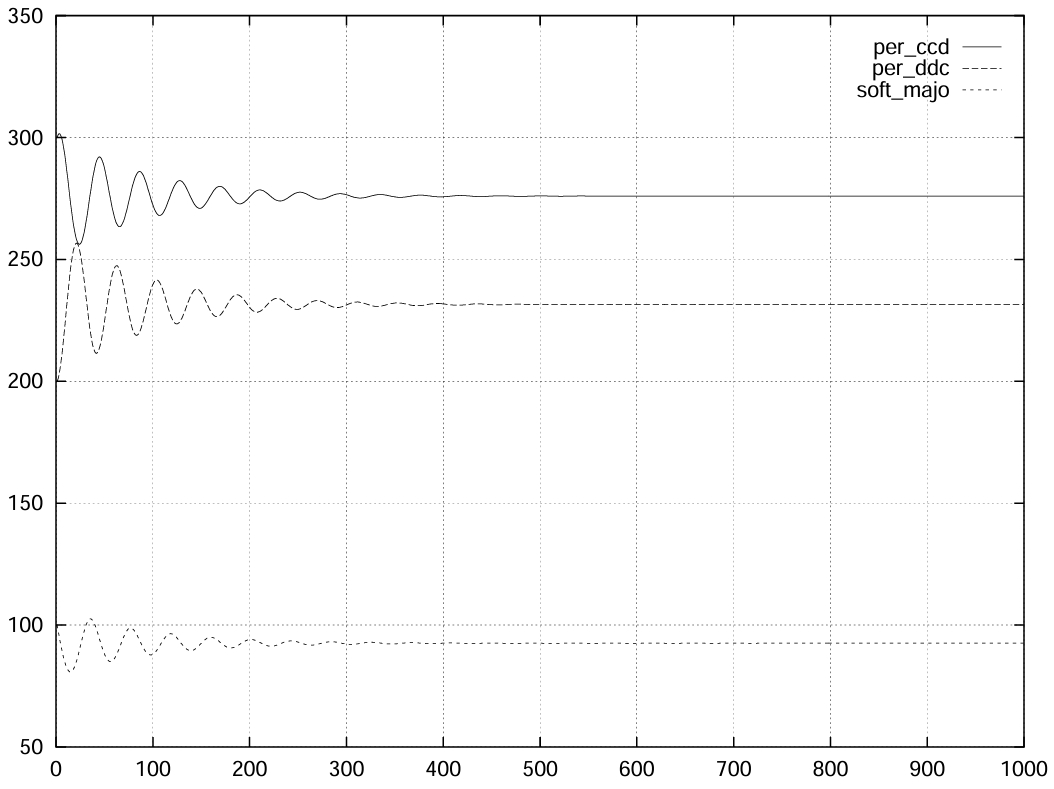
\includegraphics[width=0.49\textwidth]{RefPaperFigures/fig11b.jpeg}\par\vspace{0.5em}\par\vspace{0.5em}
	    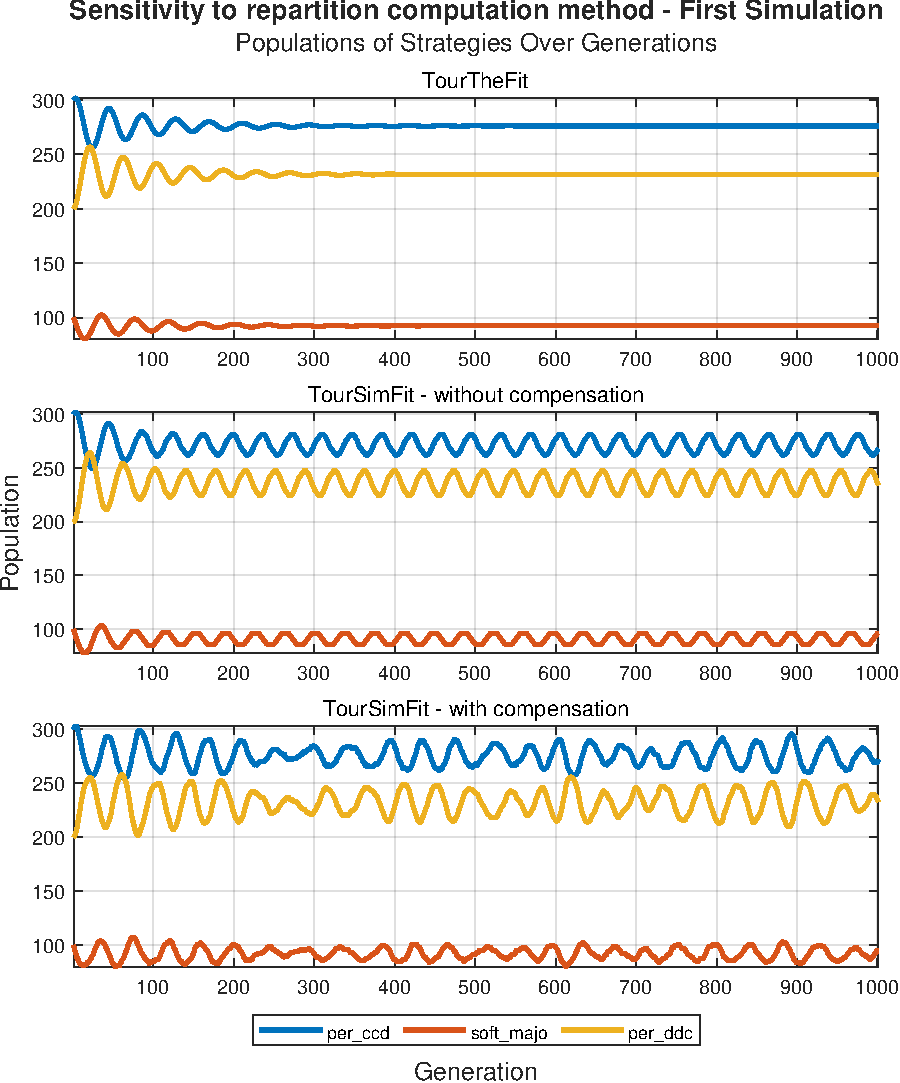
\includegraphics[width=0.7\textwidth]{Sensitivity to repartition computation method - First Simulation.pdf}
	    \caption{15th Simulation - Sensitivity to repartition computation method - First Simulation}
	    \label{fig:Sensitivity to repartition computation method - First Simulation}
	\end{figure}
\subsubsection{16th Simulation - Sensitivity to repartition computation method - Second Simulation}
This final pair of simulations again showcases the sensitivity to the repartition computation method, this time by keeping the ratios between strategies constant but by changing the actual population each strategy initially has. The results (Figure~\ref{fig:Sensitivity to repartition computation method - Second Simulation}) are exactly the same in all cases, also matching the results by Mathieu et al. Run example16 of the Examples folder (after reading Quickstart guide) to recreate the figure.
	\begin{figure}[h]
	    \centering
		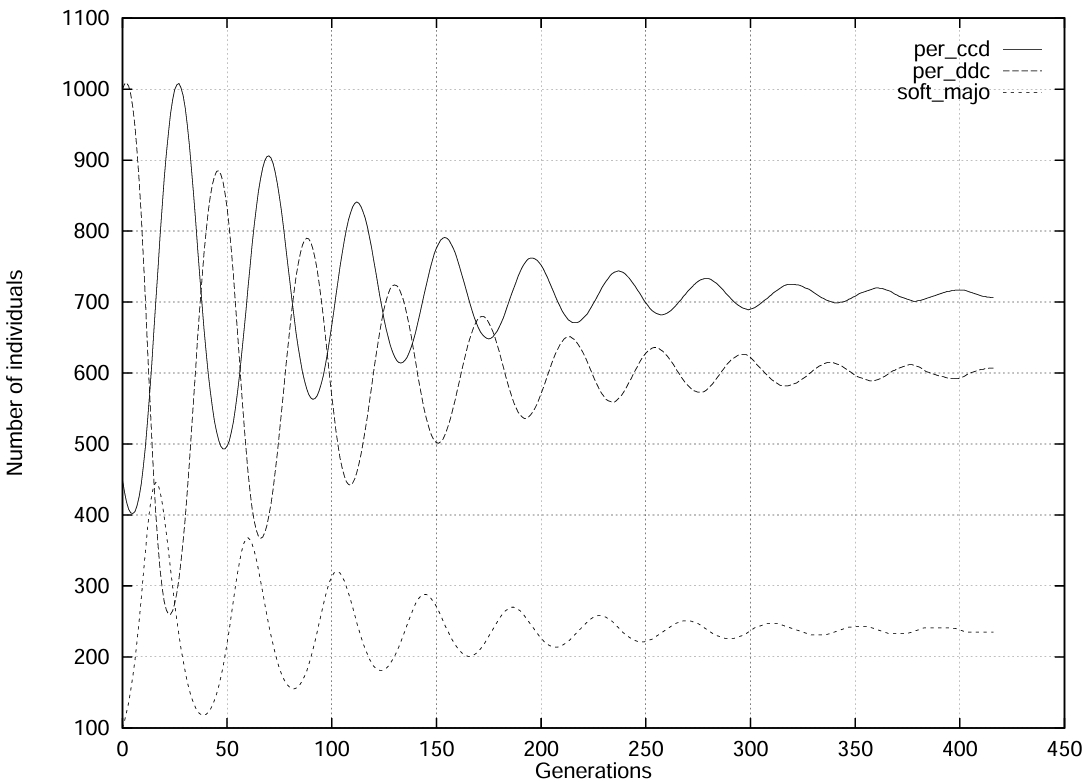
\includegraphics[width=0.7\textwidth]{RefPaperFigures/fig12a.jpeg}\par\vspace{0.5em}
	    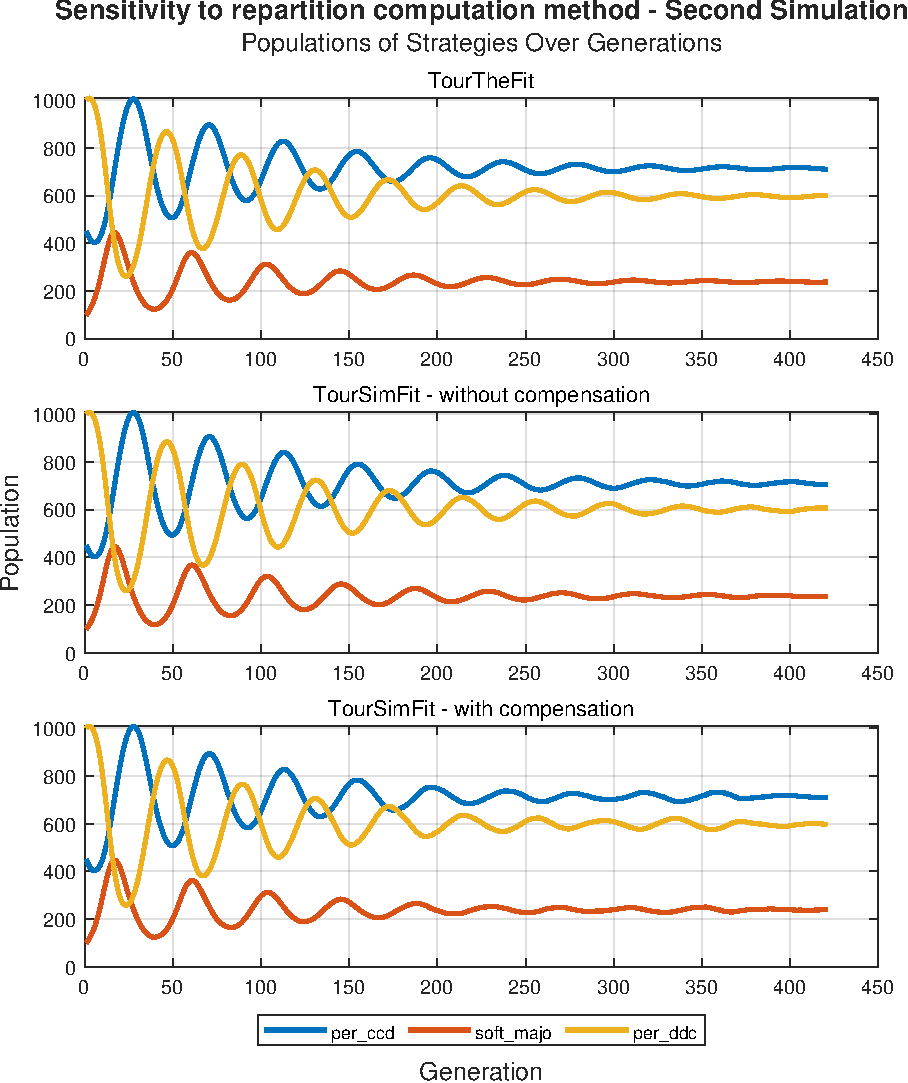
\includegraphics[width=0.7\textwidth]{Sensitivity to repartition computation method - Second Simulation.pdf}
	    \caption{16th Simulation - Sensitivity to repartition computation method - Second Simulation}
	    \label{fig:Sensitivity to repartition computation method - Second Simulation}
	\end{figure}
\subsubsection{17th Simulation - Sensitivity to repartition computation method - Third Simulation}
Lastly, all initial populations of the previous simulation are divided by 10 (thus keeping the ratios of strategies constant). This results in an increasing oscillation in the paper by Mathieu et al. The figure created (Figure~\ref{fig:Sensitivity to repartition computation method - Third Simulation}) shows the same result in the case of TourSimFit wihout compensation, but in the other two cases the dynamics constructed remain attenuated oscillations. Thus, it is once again proven that the method used to calculate the population of the next generation is one of (if not the) most importants aspect in terms of how much the results may differ. Also, it is shown that the ratio between strategies is not always enough to determine the ensuing dynamics; in some cases, such as this, the dynamics are vastly different, just by changing the magnitudes of the populations, not their ratio (from attenuated to increasing oscillations). Run example17 of the Examples folder (after reading Quickstart guide) to recreate the figure.
	\begin{figure}[h]
	    \centering
		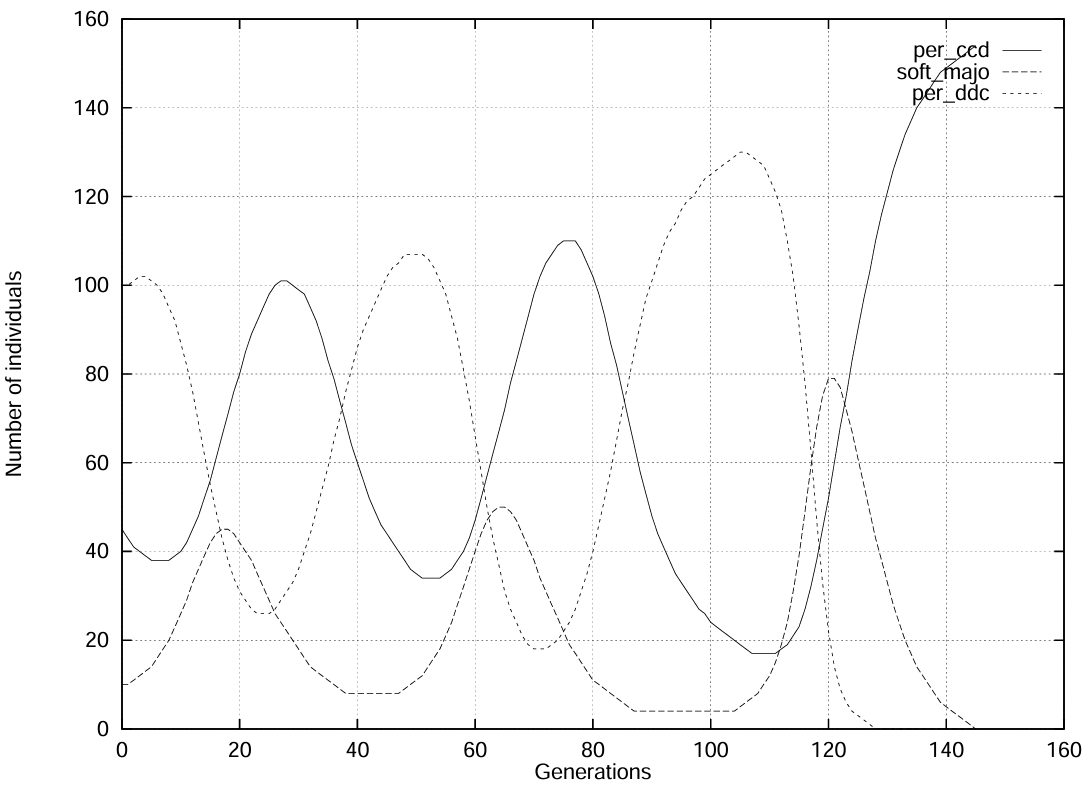
\includegraphics[width=0.7\textwidth]{RefPaperFigures/fig12b.jpeg}\par\vspace{0.5em}
	    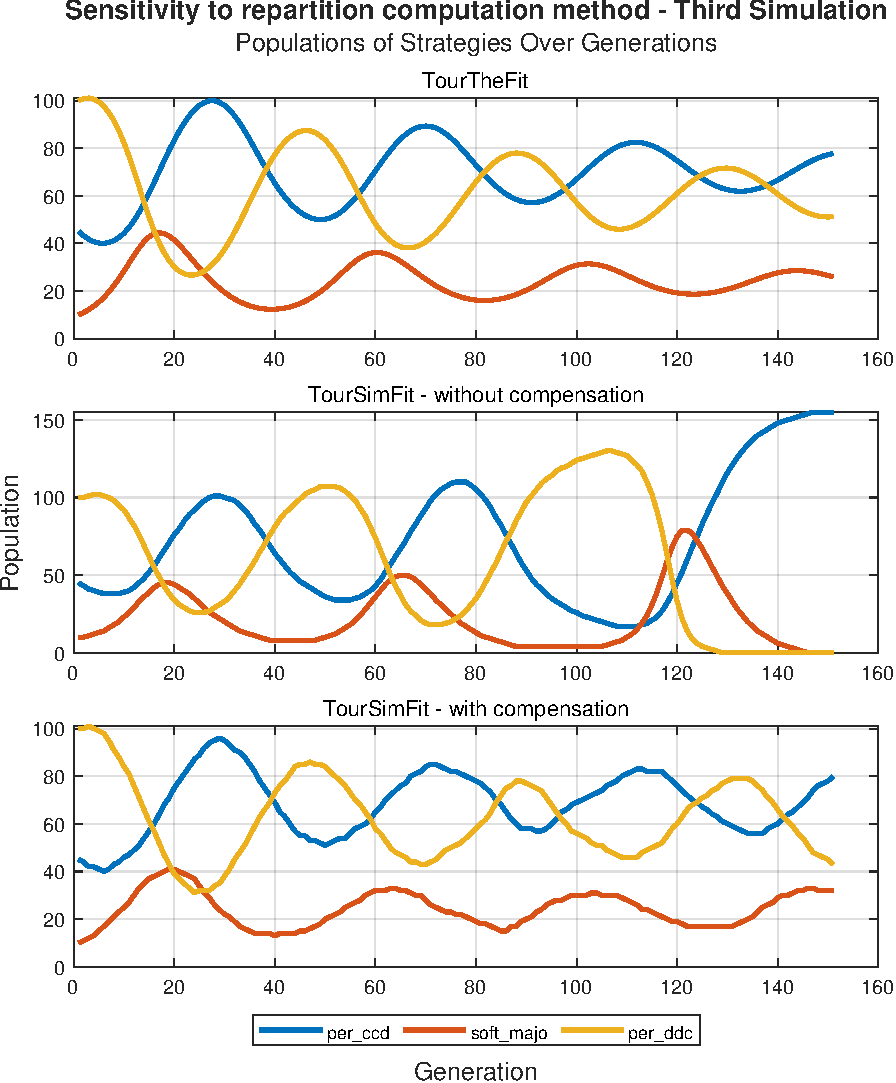
\includegraphics[width=0.7\textwidth]{Sensitivity to repartition computation method - Third Simulation.pdf}
	    \caption{17th Simulation - Sensitivity to repartition computation method - Third Simulation}
	    \label{fig:Sensitivity to repartition computation method - Third Simulation}
	\end{figure}
\subsection{Discussion}

From the above, the following final conclusions emerge regarding the evolutionary \textit{Fitness Dynamics}:

\begin{enumerate}
    \item Mathieu et al.\ appear to have used a simple floor function when calculating new populations after each generation, as this method yielded results closest to ours.

    \item In many cases of generally unstable behaviors, the diagrams differ to an observable degree depending on whether the function \texttt{TourTheFit} or the function \texttt{TourSimFit} is used, with or without compensation. This is due to the fact that many of the resulting diagrams are highly sensitive, and even a small change in the dynamics logic can significantly alter the results.

    \item The resulting diagram depends on the initial population values, the strategies used, and the payoff matrix. Even if two of these factors remain the same, a change in one of them can lead to drastically different results (even different rankings, as seen in Figure~\ref{fig:Increasing oscillations}).

    \item Assigning the remaining population members randomly according to the logic of compensation seems to be a good choice, especially given its simplicity, as it does not significantly alter the results (strategies that theoretically die out actually do die out; in general, the population tendencies do not change). Depending on the specific case being examined, it resembles either the \texttt{TourTheFit} case or the \texttt{TourSimFit} case without compensation.

    \item In general, the discrete nature of the \texttt{TourSimFit} simulations, with or without compensation, leads over time either to recurring oscillations or convergence to certain final population values. Chaos cannot really be achieved; even in Figure~\ref{fig:Disordered oscillations}, the populations eventually converge to the values predicted by \texttt{TourTheFit}. However, this does not prevent us from generating the interesting results seen in the paper.
    
    \item The results depend on many factors including the game length, the payoff matrix, the initial population (both ratio and magnitude) and the repartition computation method.
\end{enumerate}